\documentclass[a4paper]{report}
% \counterwithout{figure}{chapter} % pour compter la Figure 1 au lieu de Figure 1.1
%====================== PACKAGES ======================
\usepackage[round,authoryear]{natbib}
\usepackage[french]{babel}
\usepackage{xcolor}
% \usepackage[utf8]{inputenc}
\frenchsetup{StandardItemLabels=true}
%pour gérer les positionnement d'images
\usepackage{float}
\usepackage{amsmath}
\usepackage{graphicx}
\usepackage[colorinlistoftodos]{todonotes}
\usepackage{url}
%pour les informations sur un document compilé en PDF et les liens externes / internes
\usepackage{hyperref}
%pour la mise en page des tableaux
\usepackage{array}
\usepackage{tabularx}
%pour utiliser \floatbarrier
%\usepackage{placeins}
%\usepackage{floatrow}
%espacement entre les lignes
\usepackage{setspace}
%modifier la mise en page de l'abstract
\usepackage{abstract}
%police et mise en page (marges) du document
%\usepackage{polyglossia}
%\setmainlanguage{french}
%\setotherlanguage[variant=polytonic]{greek}
%\newfontfamily{\greekfont}[Ligatures=TeX]{Linux Libertine O}
\usepackage[T1]{fontenc}
\usepackage[top=2cm, bottom=2cm, left=3cm, right=3cm]{geometry}
%Pour les galerie d'images
\usepackage{subfig}
\usepackage{fancyhdr}
\pagestyle{fancy}
\fancyhf{}
\fancyhead[L]{\rightmark}
\fancyhead[R]{\thepage}
\renewcommand{\headrulewidth}{0.4pt}% Default \headrulewidth is 0.4pt
\renewcommand{\footrulewidth}{0.4pt}% Default \footrulewidth is 0pt

% renommer « Fig. » en « Figure »
\addto\captionsfrench{\renewcommand{\figurename}{\textsc{Figure}}}

\usepackage{lipsum} 
\usepackage{titlesec, blindtext, color}
\definecolor{gray75}{gray}{0.75}
\newcommand{\hsp}{\hspace{20pt}}
\titleformat{\chapter}[hang]{\Huge\bfseries}{\thechapter\hsp\textcolor{gray75}{|}\hsp}{0pt}{\Huge\bfseries}
%====================== INFORMATION ET REGLES ======================

%rajouter les numérotation pour les \paragraphe et \subparagraphe
\setcounter{secnumdepth}{4}
\setcounter{tocdepth}{4}

% ajouter de l'espace entre le numéro de la footnote et le texte de la footnote
\usepackage[hang]{footmisc}
\setlength{\footnotemargin}{2mm}

\usepackage{etoolbox}
\gappto{\UrlBreaks}{\UrlOrds}
\hypersetup{							% Information sur le document
pdfauthor = {Premier Auteur,
			Deuxième Auteur,
			Troisième Auteur,
    		Quatrième Auteur},			% Auteurs
pdftitle = {Nom du Projet -
			Sujet du Projet},			% Titre du document
pdfsubject = {Mémoire de Projet},		% Sujet
pdfkeywords = {Tag1, Tag2, Tag3, ...},	% Mots-clefs
pdfstartview={FitH},
    colorlinks=true,
    linkcolor=black,
    filecolor=magenta,      
    urlcolor=blue,
    citecolor=black,
    linkbordercolor=red,
    citebordercolor=red,
    urlbordercolor=red,
    pdftitle={Overleaf Example},
    pdfpagemode=FullScreen}					% ajuste la page à la largueur de l'écran
%pdfcreator = {MikTeX},% Logiciel qui a crée le document
%pdfproducer = {}} % Société avec produit le logiciel
\usepackage{fancyhdr}% http://ctan.org/pkg/fancyhdr
% \pagestyle{fancy}% Change page style to fancy
% \fancyhf{}% Clear header/footer
% \fancyhead[C]{}
% \fancyfoot[C]{}% \fancyfoot[R]{\thepage}

%======================== DEBUT DU DOCUMENT ========================

\begin{document}

%régler l'espacement entre les lignes
\newcommand{\HRule}{\rule{\linewidth}{0.5mm}}

%page de garde
%\begin{titlepage}
\begin{center}

% Upper part of the page. The '~' is needed because only works if a paragraph has started.

\includegraphics[width=0.35\textwidth]{img/unige_lettres_logo.png}~\\[1cm]

% \textsc{\LARGE Université de Genève\\Faculté des Lettres\\
% Département de linguistique}\\[1.5cm]
\Large \textsc{Université de Genève}\\Faculté des Lettres\\
Département de linguistique

\textsc{\Large }\\[0.5cm]

% Title
\HRule \\[0.4cm]

{\huge \bfseries Analyse des champs lexicaux dans le fonds patrimonial de Jean-Martin Charcot \\[0.4cm] }

\HRule \\[1.5cm]
\large{Mémoire présenté en vue de l’obtention du\medskip

\Large \textit{Certificat de spécialisation en Linguistique (CS)}\vspace{2cm}}

% Author and supervisor
\begin{minipage}{1\textwidth}
\begin{flushleft} \large
\emph{Étudiante:}\\
\textbf{Ljudmila} \textsc{\textbf{PETKOVIC}}\\
\small{N° de matricule : 19-337-757\\\href{mailto:ljudmila.petkovic@etu.unige.ch}{ljudmila.petkovic@etu.unige.ch}}
\end{flushleft}
\end{minipage}
\begin{minipage}{1\textwidth}
\begin{flushright} \large
\emph{Directeur :} \\
\textbf{Prof. D\textsuperscript{r} Christopher} \textsc{\textbf{LAENZLINGER}}

\medskip
\emph{Co-encadrant :} \\
\textbf{Dr Luka} \textsc{\textbf{NERIMA}}
\end{flushright}
\end{minipage}

\vfill

% Bottom of the page
{\large \today}

\end{center}
\end{titlepage} % ici mettre la page de garde de SU

%page blanche
\newpage
~
%ne pas numéroter cette page
\thispagestyle{empty}
\newpage
\setcounter{page}{0}
\chapter*{Remerciements}

\thispagestyle{empty}
\setcounter{page}{0}
%ne pas numéroter le sommaire
\newpage
~
\thispagestyle{empty}
\setcounter{page}{0}
%ne pas numéroter le sommaire

\newpage



%\begin{abstract}
%\hskip7mm
%%
%\begin{spacing}{1.3}
Ce projet de thèse, à la jonction des Lettres (histoire des sciences) et de l'informatique, propose une étude interdisciplinaire centrée sur la valorisation du fonds patrimonial de Jean-Martin Charcot, fondateur de la neurologie moderne au XIX\ieme{} siècle en France, au prisme des humanités numériques (\textsc{HN}) et du traitement automatique des langues (\textsc{TAL}). Plus concrètement, cette recherche se concentre sur l'exploration de la circulation des savoirs, à travers les reprises des théories scientifiques de Charcot sous forme de concepts médicaux dans ses propres écrits et dans ceux d'autres scientifiques. Ce travail vise à établir un protocole permettant d'appréhender la circulation de concepts de manière automatisée. La première contribution de ce travail est la constitution d'un corpus numérique à partir des archives en question déjà numérisées. Comme deuxième contribution, nous proposons la mise en place d'une chaîne de traitement semi-automatique consistant en l'océrisation, la correction de sortie OCR, la structuration des données au format XML-TEI, la fouille sémantique et l'alignement des textes pour étudier le transfert interdisciplinaire du discours médical de Charcot dans les écrits réalisés en collaboration et dans ceux de ses continuateurs et disciples. Ces traitements nous permettront de produire une transcription interrogeable dans notre cadre de recherche. Au-delà des finalités de ce projet de thèse, ce modèle généralisable sera aussi applicable à d'autres projets de numérisation et de valorisation des fonds patrimoniaux.

\textbf{Mots-clés} : Jean-Martin Charcot ; humanités numériques ; traitement automatique des langues ; extraction des phrases-clés.

%Au-delà du cas de Charcot, ce travail vise à établir un protocole permettant d'appréhender la circulation de concepts de manière automatisée.

\centredchapter{Abstract}
%
%\end{spacing}
%\end{abstract}

\thispagestyle{empty}
\setcounter{page}{0}
%ne pas numéroter le sommaire
\newpage
~
\thispagestyle{empty}
\setcounter{page}{0}
%ne pas numéroter le sommaire

\newpage

\tableofcontents
\thispagestyle{empty}
\setcounter{page}{0}
%ne pas numéroter le sommaire

\newpage

%espacement entre les lignes d'un tableau
\renewcommand{\arraystretch}{1.5}

%====================== INCLUSION DES PARTIES ======================

~
\thispagestyle{empty}
%recommencer la numérotation des pages à "1"
\setcounter{page}{0}
\newpage



\chapter{Introduction}
\minitoc% Creating an actual minitoc

%\begin{itemize}
%\item 10-60 pages (10\% du total de la thèse)
%\end{itemize}

%Feuille de route :
%\begin{enumerate}
%\item accroche
%\item présentation globale du sujet
%\item SotA, cadre théorique de la thèse
%\item problématique
%\item hypothèses
%\item méthodo du recueil de données
%\item motivations, objectif de l'étude, portée
%\item annonce du plan
%\end{enumerate}


%\section{Enjeux et motivations}
%\begin{itemize}
%\item présentation du sujet et de la problématique
%\end{itemize}



L’intérêt pour ce parcours doctoral s'ancre dans les expériences de l'autrice en valorisation numérique de ressources textuelles variées, menées lors du master en \og Informatique pour les sciences humaines \fg{}\footnote{\url{http://arhiva.rect.bg.ac.rs/en/education/interdisciplinary/computing.php}} à l'université de Belgrade et du certificat de spécialisation en linguistique\footnote{\url{https://www.unige.ch/lettres/linguistique/program/postgrade}} à Genève. Ces travaux ont porté sur des corpus tels que les paroles de chansons rock d’ex-Yougoslavie \citep{petkovic2019creation}, les manuscrits de M\textsuperscript{me} de Sévigné (\citealp{gabay2020quantifying,gabay2021katabase})\footnote{Projet \textit{Katabase} : \url{https://katabase.huma-num.fr/}}, ou encore les catalogues d’expositions\footnote{Projet \textit{Virtual Contagions} : \url{https://www.unige.ch/visualcontagions/}}.
À ces projets s'ajoute le stage effectué au sein de l'équipe-projet Observatoire des Textes, des Idées et des Corpus (\textsc{ObTIC})\footnote{\url{https://obtic.sorbonne-universite.fr/presentation/}.} de Sorbonne Université entre le 29 mars 2021 et le 31 juillet 2021, sous l'encadrement de Prof. D\textsuperscript{r} Glenn Roe et D\textsuperscript{r} Motasem Alrahabi, ingénieur de recherche. Dans le cadre du projet de la Très Grande Bibliothèque (\textsc{TGB})\footnote{\url{http://obvil.lip6.fr/tgb}}, l'enjeu de ce stage a été d'exploiter le corpus constitué d'un grand volume de documents \textsc{XML-TEI} en français, OCRisés\footnote{Forme francisée dérivée de l'abréviation anglaise \textsc{OCR} pour \textit{optical character recognition}, soit \og{}reconnaissance optique de caractères\fg{}.} (transcrits automatiquement) et non corrigés, issus des collections Gallica de la Bibliothèque nationale de France (\textsc{BnF}). 
À l'issue du stage, le projet de recherche doctoral a été mis en place lors de la campagne d'attribution de contrats doctoraux 2021 par l'institut Observatoire des patrimoines de l'Alliance Sorbonne Université (\textsc{OPUS})\footnote{\url{https://institut-opus.sorbonne-universite.fr/node/478}}. 

Ce projet vise à répondre aux enjeux portés par l'\textsc{OPUS}, ainsi qu'à ceux de la Bibliothèque de neurosciences Jean-Martin Charcot -- rattachée à la Bibliothèque de Sorbonne Université (\textsc{BSU})\footnote{\url{https://www.sorbonne-universite.fr/bu/decouvrir-nos-bibliotheques/la-bibliotheque-charcot}} et détentrice du fonds patrimonial de Jean-Martin Charcot -- dans une perspective de valorisation de ce fonds. Plus globalement, cette thèse entend s'inscrire dans les dynamiques de la communauté des \textsc{HN}, dont les travaux portent sur les objets patrimoniaux sous toutes leurs formes : (im)matériels, culturels ou naturels. Au carrefour de l'histoire des sciences et de la linguistique computationnelle, ce projet fait également partie des travaux de l'axe \#3 qui sont menés par l'équipe-projet \textsc{ObTIC} et qui sont tournés vers le dialogue constant entre les recherches qualitatives et quantitatives. 

La motivation à poursuivre ce travail de recherche découle d’une part de l'abondance des études consacrées à la valorisation des archives patrimoniales et aux repérages des circulations culturelles et intellectuelles (voir section~\ref{sect:sota_circulations}). Elle s'appuie également sur la confusion que suscite le terme \textit{circulation des savoirs}, souvent méconnu des chercheur$\cdot$se$\cdot$x$\cdot$s ne travaillant pas dans le domaine du \textsc{TAL} ou des \textsc{HN}.
Cette barrière disciplinaire est apparue de manière particulièrement tangible lors des échanges de l’autrice avec les spécialistes de Charcot en médecine, histoire des sciences et critique littéraire. C'est pourquoi cette thèse entend constituer un pas vers la démystification des méthodes quantitatives, mises au service des recherches en histoire des sciences et plus largement en sciences humaines et sociales (ci-après \og{}\textsc{SHS}\fg{}).

\section{Un projet pour pister numériquement la circulation des savoirs}
Ce projet de thèse propose une étude interdisciplinaire centrée sur la valorisation du fonds patrimonial de Jean-Martin Charcot, fondateur de la neurologie moderne au XIX\textsuperscript{e} siècle en France, au prisme des humanités numériques (\textsc{HN}) et du traitement automatique des langues (\textsc{TAL}). Nous nous intéressons à l'analyse de la genèse et de la migration des savoirs médicaux de Charcot en pathologie anatomique, neurologie et psychologie. Plus concrètement, cette recherche se concentre sur l'exploration de la circulation des savoirs à travers les reprises des théories scientifiques de Charcot sous forme de concepts médicaux dans les écrits co-rédigés par Charcot ainsi que dans ceux de ses disciples, collaborateurs et successeurs constituant son \og{}réseau scientifique\fg{}. Le présent mémoire vise également à approfondir les recherches issues du travail de \citet{petkovic2023circulation} s'inscrivant dans l'optique de l'exploration quantitative de ce type de circulation. 
 Si l'importance des contributions scientifiques de Charcot est un sujet largement étudié du point de vue de l'histoire des neurosciences (\citealp{bogousslavsky2011following,broussolle2012,camargo2024}, parmi de nombreux autres travaux), cet aspect reste inexploré dans une perspective quantitative. Cela n'est pas très étonnant, étant donné que l'étude des textes dans les archives en ligne reste un domaine en cours de développement dans un contexte de circulation des connaissances \citep[p.~4]{milia2023}.
%Dans le cadre de cette thèse, nous nous intéressons à la circulation à travers l'analyse de la genèse et de la migration du discours médical -- en pathologie anatomique, neurologie et psychologie -- dans les écrits co-rédigés par Charcot ainsi que dans ceux de ses disciples, collaborateurs et successeurs constituant son \og{}réseau scientifique\fg{}. Si l'importance des contributions scientifiques de Charcot est un sujet largement étudié du point de vue de l'histoire des neurosciences (\citealp{bogousslavsky2011following,broussolle2012,camargo2024}, parmi de nombreux autres travaux), cet aspect reste inexploré dans une perspective quantitative. Cela n'est pas très étonnant, étant donné que l'étude des textes dans les archives Internet et des données en ligne dans un contexte de circulation des connaissances en général reste un domaine en cours de développement \citep{milia2023}. À ce titre, nous nous tâchons à mesurer informatiquement l'impact des travaux de Charcot sur son réseau scientifique. Cette mesure se fonde sur l'analyse des concepts-clés en matière de son discours scientifique, et plus particulièrement sur l'opérationnalisation du terme \og{}influence\fg{}, définie ici comme une intertextualité uni-directionnelle, allant des écrits de Charcot (ci-après corpus \og{}Charcot\fg{}) vers ceux de son réseau scientifique (ci-après corpus \og{}Autres\fg{}). Il s'agit donc \textit{in fine} d'aborder computationnellement la question des circulations, non pas des artefacts matériels comme les manuscrits \citep{gabay2021katabase} et les images \citep{joyeux2019visual}, mais des phénomènes textuels complexes \citep{manjavacas} ayant une dimension théorique forte. 


Dans le cadre de l'analyse numérique de l'impact scientifique de Charcot, nous étudions \textit{in fine} la circulation de ses théories et des concepts médicaux dont il était inventeur (p. ex. \textit{sclérose latérale amyotrophique} -- \textit{SLA}) et transmetteur (p. ex. \textit{hystérie})\footnote{En effet, Charcot n'a pas inventé ce terme, mais en réinterprété le sens. Pour une discussion détaillée sur l'évolution de ce terme, voir la partie \ref{hysterie}.}. Cette démarche nous oblige de :
\begin{enumerate}
	\item formaliser en premier lieu la définition du terme \textit{concept scientifique}, identifiable dans un corpus numérique, tout en prenant en compte les difficultés inhérentes à la définition d'un concept \textit{per se}, ainsi qu'à celle de ses termes apparentés : \textit{idée}, \textit{terme}, \textit{mot} ou \textit{mot-clé} (parties \ref{concept} et \ref{termes}) ;
	\item comprendre, conceptualiser et opérationnaliser \og{}comment des concepts, des théories ou des méthodes circulent, s'échangent, s'empruntent, se transfèrent et se transforment dans le passage d'une discipline à une autre\fg{}, questionnement partagé avec \citeauthor{landais2014frederic} (\citeyear{landais2014frederic}, p.~331) (partie \ref{sect:modalites_circulations}).
\end{enumerate}

%Le pré-requis pour analyser ce type de circulation est de formaliser les concepts scientifiques identifiables dans notre corpus d'étude.
Cela est intrinsèquement lié au double objectif de cette thèse, car nous souhaitons :
\begin{itemize} 
	\item formaliser une approche numérique pour tracer l'évolution des concepts médicaux en général ;
	\item en prenant comme cas d'étude les archives de Charcot, pister numériquement la circulation des savoirs médicaux dans la communauté scientifique de son époque.
\end{itemize}
\medskip


%\section{Enjeux et motivations}
%\begin{itemize}
%\item présentation du sujet et de la problématique
%\end{itemize}






\section{La complexité du terme \og{}circulation des savoirs\fg{}}
\label{sect:modalites_circulations}
Les savoirs participent à un double mouvement d'héritage et de transmission. En effet, leur circulation sur le temps long reflète ces dynamiques de transmission, essentielles à la formation de courants de pensée, ainsi qu'à l'affirmation d’une identité construite autour d'un savoir partagé \citep[p.~251]{adell2011chapitre}. Dans une perspective contemporaine, de nombreux$\cdot$ses chercheur$\cdot$se$\cdot$s$\cdot$x partagent le point de vue selon lequel la notion de circulation des savoirs constitue un champ de recherche vaste, ainsi qu'un nouveau paradigme de la connaissance depuis le début du XXI\ieme{} siècle et l'avènement du Web \textsc{2.0} (\citealp{landais2014frederic,quet2014frederic}). Cette phase de l'évolution du Web se caractérisait notamment par la transformation majeure de l'Internet en vue du développement des réseaux sociaux, des blogs et des sites participatifs, tout en permettant aux utilisateur$\cdot$trice$\cdot$s$\cdot$x de créer, partager et interagir avec du contenu Web. Nous traversons actuellement l'ère du Web \textsc{3.0}, né dans les années 2010 et appelé également \og{}Web sémantique\fg{}, qui permet de lier et structurer l'information afin d'en extraire la connaissance (\citeauthor{andrade2013sociologie} \citeyear{andrade2013sociologie}, p.~107). Par ailleurs, \citeauthor{landais2014frederic} (\citeyear{landais2014frederic}, p.~331) remarque que ce type de circulation connaît une croissance importante grâce aux outils de la numérisation de la production scientifique et de l'édition numérique des ouvrages.
%les savoirs sont amenés à circuler, à voyager, à se propager, mais aussi à communiquer plus rapidement ce qui ouvre de nombreuses pistes de recherche, aussi bien théoriques qu'appliquées, orientées vers l'exploration de la nature de ces circulations. 

Le terme en question reste toutefois assez complexe en raison de visions différentes sur la façon de le définir. Afin d'éclairer cette problématique, \citeauthor{quet2014frederic} (\citeyear{quet2014frederic}, pp.~221--222) souligne trois aspects suivants :
\begin{enumerate}
	\item \textbf{Éléments de la circulation}. Qu'est-ce qui circule ? 
	\begin{itemize}
		\item individus (savants, techniciens, traducteurs, etc.) ;
		\item objets matériels (instruments scientifiques, ouvrages etc.) :
		\item constructions symboliques (théories, concepts etc.).
	\end{itemize}  
	\item \textbf{Conceptions de la circulation et méthodes de son analyse} ;
	\begin{itemize}
		\item définition de la circulation comme \og{}traduction\fg{}, \og{}diffusion\fg{}, \og{}accès\fg{} ou \og{}succès\fg{} ;
		\item critères méthodologiques possibles pour étudier la circulation p. ex. d'une théorie : 
		\begin{itemize}
			\item circulations géographiques des principaux concepteurs qu'on lui reconnaît ;
			\item circulations et lectures des textes produits par leurs concepteurs ;
			\item usages et applications analogiques qui en sont faits dans d'autres domaines.
		\end{itemize} 
		\item enjeux d'articulation de ces différents niveaux d'observation du point de vue méthodologique et de celui de la production du texte de recherche, dans le cas des croisements de ces niveaux.
	\end{itemize}
	\item \textbf{Conceptions analytiques et normatives des savoirs}
	\begin{itemize}
		\item affaiblissement des catégories des \og{}savoirs profanes\fg{} et \og{}savoirs scientifiques\fg{}, ainsi que de l'opposition entre eux ;
		\item revalorisation des savoirs implicites et de la dimension pratique des connaissances ;
		\item glorification de la circulation comme porteuse de valeurs \textit{a priori} positives : confrontation à l'autre, hybridation, production de nouveauté, etc.
	\end{itemize}
\end{enumerate}


%\section{Modalités des circulations des savoirs}
%De nombreux$\cdot$ses chercheur$\cdot$se$\cdot$s$\cdot$x partagent le point de vue selon lequel la notion de circulation des savoirs constitue un champ de recherche vaste, ainsi qu'un nouveau paradigme de la connaissance depuis le début du XXI\ieme{} siècle et l'avènement du Web \textsc{2.0} (\citealp{landais2014frederic,quet2014frederic}). Cette phase de l'évolution du Web se caractérisait notamment par la transformation majeure de l'Internet en vue du développement des réseaux sociaux, des blogs et des sites participatifs, tout en permettant aux utilisateur$\cdot$trice$\cdot$s$\cdot$x de créer, partager et interagir avec du contenu Web. Nous traversons actuellement l'ère du Web \textsc{3.0}, né dans les années 2010 et appelé également \og{}Web sémantique\fg{}, qui permet de lier et structurer l'information afin d'en extraire la connaissance (\citeauthor{andrade2013sociologie} \citeyear{andrade2013sociologie}, p.~107). Néanmoins, en se référant à la circulation des savoirs, \citeauthor{landais2014frederic} (\citeyear{landais2014frederic}, p.~331) remarque que ce phénomène connaît une croissance importante grâce aux outils de la numérisation de la production scientifique et de l'édition numérique des ouvrages.
%%les savoirs sont amenés à circuler, à voyager, à se propager, mais aussi à communiquer plus rapidement ce qui ouvre de nombreuses pistes de recherche, aussi bien théoriques qu'appliquées, orientées vers l'exploration de la nature de ces circulations. 
%
%Le terme en question reste toutefois assez complexe en raison de visions différentes sur la façon de le définir. Afin d'éclairer cette problématique, \citeauthor{quet2014frederic} (\citeyear{quet2014frederic}, pp.~221--222) souligne trois aspects suivants :
%\begin{enumerate}
%	\item \textbf{Éléments de la circulation}. Qu'est-ce qui circule ? 
%	\begin{itemize}
%		\item individus (savants, techniciens, traducteurs, etc.) ;
%		\item objets matériels (instruments scientifiques, ouvrages etc.) :
%		\item constructions symboliques (théories, concepts etc.).
%	\end{itemize}  
%	\item \textbf{Conceptions de la circulation et méthodes de son analyse} ;
%	\begin{itemize}
%		\item définition de la circulation comme \og{}traduction\fg{}, \og{}diffusion\fg{}, \og{}accès\fg{} ou \og{}succès\fg{} ;
%		\item critères méthodologiques possibles pour étudier la circulation p. ex. d'une théorie : 
%		\begin{itemize}
%			\item circulations géographiques des principaux concepteurs qu'on lui reconnaît ;
%			\item circulations et lectures des textes produits par leurs concepteurs ;
%			\item usages et applications analogiques qui en sont faits dans d'autres domaines.
%		\end{itemize} 
%		\item enjeux d'articulation de ces différents niveaux d'observation du point de vue méthodologique et de celui de la production du texte de recherche, dans le cas des croisements de ces niveaux.
%	\end{itemize}
%	\item \textbf{Conceptions analytiques et normatives des savoirs}
%	\begin{itemize}
%		\item affaiblissement des catégories des \og{}savoirs profanes\fg{} et \og{}savoirs scientifiques\fg{}, ainsi que de l'opposition entre eux ;
%		\item revalorisation des savoirs implicites et de la dimension pratique des connaissances ;
%		\item glorification de la circulation comme porteuse de valeurs \textit{a priori} positives : confrontation à l'autre, hybridation, production de nouveauté, etc.
%	\end{itemize}
%\end{enumerate}
%
%Dans le cadre de l'analyse numérique de l'impact scientifique de Charcot, nous étudions \textit{in fine} la circulation de ses théories et des concepts médicaux dont il était inventeur (p. ex. \textit{SLA}) et transmetteur (p. ex. \textit{hystérie})\footnote{Comme déjà expliqué dans la partie \ref{hysterie}, Charcot n'a pas inventé ce terme, mais en réinterprété le sens.}. Cette démarche nous oblige de :
%\begin{enumerate}
%	\item formaliser en premier lieu la définition du terme \textit{concept scientifique}, identifiable dans un corpus numérique, tout en prenant en compte les difficultés inhérentes à la définition d'un concept \textit{per se}, ainsi qu'à celle de ses termes apparentés : \textit{idée}, \textit{terme}, \textit{mot} ou \textit{mot-clé} (parties \ref{concept} et \ref{termes}) ;
%	\item comprendre, conceptualiser et opérationnaliser \og{}comment des concepts, des théories ou des méthodes circulent, s'échangent, s'empruntent, se transfèrent et se transforment dans le passage d'une discipline à une autre\fg{}, questionnement partagé avec \citeauthor{landais2014frederic} (\citeyear{landais2014frederic}, p.~331) (partie \ref{circulations}).
%\end{enumerate}

Dans le cadre de notre étude, le terme \og{}circulation des savoirs\fg{} est entendu comme la diffusion des constructions symboliques (théories et concepts scientifiques) produites par leur concepteur (Charcot) et repérées dans les ouvrages de son réseau. Ainsi, le terme \og{}diffusion\fg{} englobe l'influence \textit{a priori} positive (\og{}succès\fg{}, \og{}production de nouveauté\fg{}), mais aussi la réception parfois mitigée des observations de Charcot.

%\section{Modalités des circulations des savoirs}
%De nombreux$\cdot$ses chercheur$\cdot$se$\cdot$s$\cdot$x partagent le point de vue selon lequel la notion de circulation des savoirs constitue un champ de recherche vaste, ainsi qu'un nouveau paradigme de la connaissance depuis le début du XXI\ieme{} siècle et l'avènement du Web \textsc{2.0} (\citealp{landais2014frederic,quet2014frederic}). Cette phase de l'évolution du Web se caractérisait notamment par la transformation majeure de l'Internet en vue du développement des réseaux sociaux, des blogs et des sites participatifs, tout en permettant aux utilisateur$\cdot$trice$\cdot$s$\cdot$x de créer, partager et interagir avec du contenu Web. Nous traversons actuellement l'ère du Web \textsc{3.0}, né dans les années 2010 et appelé également \og{}Web sémantique\fg{}, qui permet de lier et structurer l'information afin d'en extraire la connaissance (\citeauthor{andrade2013sociologie} \citeyear{andrade2013sociologie}, p.~107). Néanmoins, en se référant à la circulation des savoirs, \citeauthor{landais2014frederic} (\citeyear{landais2014frederic}, p.~331) remarque que ce phénomène connaît une croissance importante grâce aux outils de la numérisation de la production scientifique et de l'édition numérique des ouvrages.
%%les savoirs sont amenés à circuler, à voyager, à se propager, mais aussi à communiquer plus rapidement ce qui ouvre de nombreuses pistes de recherche, aussi bien théoriques qu'appliquées, orientées vers l'exploration de la nature de ces circulations. 
%
%Le terme en question reste toutefois assez complexe en raison de visions différentes sur la façon de le définir. Afin d'éclairer cette problématique, \citeauthor{quet2014frederic} (\citeyear{quet2014frederic}, pp.~221--222) souligne trois aspects suivants :
%\begin{enumerate}
%	\item \textbf{Éléments de la circulation}. Qu'est-ce qui circule ? 
%	\begin{itemize}
%		\item individus (savants, techniciens, traducteurs, etc.) ;
%		\item objets matériels (instruments scientifiques, ouvrages etc.) :
%		\item constructions symboliques (théories, concepts etc.).
%	\end{itemize}  
%	\item \textbf{Conceptions de la circulation et méthodes de son analyse} ;
%	\begin{itemize}
%		\item définition de la circulation comme \og{}traduction\fg{}, \og{}diffusion\fg{}, \og{}accès\fg{} ou \og{}succès\fg{} ;
%		\item critères méthodologiques possibles pour étudier la circulation p. ex. d'une théorie : 
%		\begin{itemize}
%			\item circulations géographiques des principaux concepteurs qu'on lui reconnaît ;
%			\item circulations et lectures des textes produits par leurs concepteurs ;
%			\item usages et applications analogiques qui en sont faits dans d'autres domaines.
%		\end{itemize} 
%		\item enjeux d'articulation de ces différents niveaux d'observation du point de vue méthodologique et de celui de la production du texte de recherche, dans le cas des croisements de ces niveaux.
%	\end{itemize}
%	\item \textbf{Conceptions analytiques et normatives des savoirs}
%	\begin{itemize}
%		\item affaiblissement des catégories des \og{}savoirs profanes\fg{} et \og{}savoirs scientifiques\fg{}, ainsi que de l'opposition entre eux ;
%		\item revalorisation des savoirs implicites et de la dimension pratique des connaissances ;
%		\item glorification de la circulation comme porteuse de valeurs \textit{a priori} positives : confrontation à l'autre, hybridation, production de nouveauté, etc.
%	\end{itemize}
%\end{enumerate}
%
%Dans le cadre de l'analyse numérique de l'impact scientifique de Charcot, nous étudions \textit{in fine} la circulation de ses théories et des concepts médicaux dont il était inventeur (p. ex. \textit{SLA}) et transmetteur (p. ex. \textit{hystérie})\footnote{Comme déjà expliqué dans la partie \ref{hysterie}, Charcot n'a pas inventé ce terme, mais en réinterprété le sens.}. Cette démarche nous oblige de :
%\begin{enumerate}
%	\item formaliser en premier lieu la définition du terme \textit{concept scientifique}, identifiable dans un corpus numérique, tout en prenant en compte les difficultés inhérentes à la définition d'un concept \textit{per se}, ainsi qu'à celle de ses termes apparentés : \textit{idée}, \textit{terme}, \textit{mot} ou \textit{mot-clé} (parties \ref{concept} et \ref{termes}) ;
%	\item comprendre, conceptualiser et opérationnaliser \og{}comment des concepts, des théories ou des méthodes circulent, s'échangent, s'empruntent, se transfèrent et se transforment dans le passage d'une discipline à une autre\fg{}, questionnement partagé avec \citeauthor{landais2014frederic} (\citeyear{landais2014frederic}, p.~331) (partie \ref{circulations}).
%\end{enumerate}





\chapter{Circulations numériques}
\label{sota}
\section{Modalités des circulations des savoirs}
De nombreux$\cdot$ses chercheur$\cdot$se$\cdot$s$\cdot$x partagent le point de vue selon lequel la notion de \og{}circulation des savoirs\fg{} constitue un champ de recherche vaste, ainsi qu'un nouveau paradigme de la connaissance depuis le début du XXI\ieme{} siècle et l'avènement du Web 2.0\footnote{Cette phase de l'évolution du Web se caractérise notamment par la transformation majeure de l'Internet en vue du développement des réseaux sociaux, des blogs et des sites participatifs, tout en permettant aux utilisateur$\cdot$trice$\cdot$s$\cdot$x de créer, partager et interagir avec du contenu Web. Nous traversons actuellement l'ère du Web 3.0 qui repose sur des technologies telles que la chaîne de blocs (angl. \textit{blockchain}), le \textit{NFT} (angl. \textit{non-fungible token}), l'intelligence artificielle, métavers et le Web sémantique \citep{varet2023nouvelles}.}
(\citealp{landais2014frederic,quet2014frederic}). Le terme en question reste toutefois assez complexe en raison de visions différentes sur la façon de le définir. Afin d'éclairer cette problématique, \citet{quet2014frederic} souligne trois aspects suivants\smalltodo{3 aspects} :
\begin{enumerate}
    \item \textbf{Éléments de la circulation}. Qu'est-ce qui circule ? 
    \begin{itemize}
        \item individus (savants, techniciens, traducteurs, etc.)
        \item objets matériels (instruments scientifiques, ouvrages etc.)
        \item constructions symboliques (théories, concepts etc.)
    \end{itemize}  
    \item \textbf{Conceptions de la circulation et méthodes de son analyse}
    \begin{itemize}
        \item définition de la circulation comme \og{}traduction\fg{}, \og{}diffusion\fg{}, \og{}accès\fg{} ou \og{}succès\fg{}
        \item critères méthodologiques possibles pour étudier la circulation p. ex. d'une théorie : 
        \begin{itemize}
            \item circulations géographiques des principaux concepteurs qu'on lui reconnaît
            \item circulations et lectures des textes produits par leurs concepteurs  
            \item usages et applications analogiques qui en sont faits dans d'autres domaines
        \end{itemize} 
        \item enjeux d'articulation de ces différents niveaux d'observation du point de vue méthodologique et de celui de la production du texte de recherche, dans le cas des croisements de ces niveaux
    \end{itemize}
    \item \textbf{Conceptions analytiques et normatives des savoirs}
    \begin{itemize}
        \item affaiblissement des catégories des \og{}savoirs profanes\fg{} et \og{}savoirs scientifiques\fg{}, ainsi que de l'opposition entre eux
        \item revalorisation des savoirs implicites et de la dimension pratique des connaissances
        \item glorification de la circulation comme porteuse de valeurs \textit{a priori} positives : confrontation à l'autre, hybridation, production de nouveauté, etc.
    \end{itemize}
\end{enumerate}

Dans le cadre de l'analyse de l'impact scientifique de Charcot, nous étudions \textit{in fine} la circulation de ses théories et des concepts médicaux dont il était inventeur (p. ex. \textit{SLA}) et transmetteur (p. ex. \textit{hystérie})\footnote{Comme déjà expliqué dans la sous-section \ref{hysterie}, Charcot n'a pas inventé ce terme, mais en réinterprété le sens.}. La section \ref{concept} élabore les différentes approches pour définir plus globalement la notion des concepts historiques qui nous orienteront vers une définition des concepts médicaux en particulier. \smalltodo{pont}

\section{Constitution d'un concept historique}
\label{concept}

Le mot \og{}concept\fg{} est un terme générique qui renvoie à un grand nombre de définitions provenant de divers domaines de pensée, sans qu'il en existe une qui soit exhaustive et universellement acceptée. En mathématiques et en sciences cognitives (philosophie, psychologie, intelligence artificielle etc.), un concept représente une catégorie basique axiomatique qui est indétectable et comprise de manière intuitive.\smalltodo{concept mathématique} On peut le comprendre également comme une unité de connaissance, une idée, un cadre, un script, un \textit{gestalt}\footnote{Allem. \og{}forme, figure\fg{}. Le terme provient du domaine de la psychologie de la forme (théorie de la gestalt ou gestaltisme) dans les années 1920. Selon ce courant, un individu observe les phénomènes dans leur ensemble de manière holistique, et non pas comme les parties individuelles juxtaposées ou additionnées (p. ex. cinq cercles qui se chevauchent, lesquels l'{\oe}il humain perçoit comme le logo se référant au concept des Jeux olympiques).} ou un hypéronyme d'une notion \foreignlanguage{russian}{(Лихачёв, \citeyear{lihachev1997}}). 

En revanche, selon les linguistes, un concept a une structure double, constituée du sens linguistique et culturel
%dont linguistique (générale, cognitive, psycholinguistique, ethnolinguistique), philosophie, métaphysique ou mathématiques
 \citep{nemickiene2011concept}. Sa couche intérieure est constituée du noyau étymologique sur lequel repose ensuite la couche périphérique qui hérite les éléments formés par la culture, les traditions et les expériences humaines \foreignlanguage{russian}{(Степанов, \citeyear{stepanov2007}}). En linguoculturologie, on retrouve le terme \og{}concept linguo-culturel\fg{} qui reflète cette nature double du concept. Il peut être exprimé par de différentes éléments du langage, soit : lexèmes, idiomes, collocations, phrases ou textes entiers. \smalltodo{concept linguistique} \hl{à développer}
 
 \hl{Concept / circulation en analyse du discours / TAL / HN} ?  
\begin{itemize}
\item TAL : concept = groupe de mots, créé manuellement ou extrait à partir des ontologies ou des thésaurus
\end{itemize}



Afin de pouvoir analyser les concepts médicaux liés à Charcot, il est essentiel de déterminer à partir de quel moment un mot ou un groupe de mots devient un concept en sciences humaines et sociales (ci-après SHS). Du point de vue de l'histoire des concepts (allem. \textit{Begriffsgeschichte}), cette transformation survient lorsqu'un seul mot\smalltodo{Begriffsgeschi\-chte} comprend toute la gamme des significations dérivées d'un contexte sociopolitique \citep[p. 258]{koselleck2011introduction}. À titre d'exemple, le concept d'un \textit{état} ne peut être interprété qu'à travers ses différents constituants, dont \textit{souveraineté territoriale, législation, fiscalité}, parmi maints d'autres. Les concepts sont donc les concentrations par défaut ambiguës d'une multitude de contenus sémantiques, uniquement interprétables et indéfinissables, par contraste avec des significations des mots qui peuvent être définies de manière exacte \citep[p. 20]{koselleck2011introduction}. 

De plus, les concepts comme \textit{histoire} ou \textit{progrès} sont caractérisés comme \og{}collectifs singuliers\fg{} qui marquent un passage du domain concret d'un individu (plusieurs \textit{histoires} et \textit{progrès} individuels) au domain abstrait et général du collectif social (une \textit{histoire} ou un \textit{progrès} général ou collectif). \smalltodo{collectifs singuliers} Ce phénomène linguistique, ainsi que la création des concepts comme \textit{industrie, usine, classe moyenne} etc., reflète un changement de paradigme dans l'organisation sociale survenu lors des révolutions politiques et industrielles \citep[p. 1]{hobsbawm2010age}. Cela traduit donc le lien fort entre l'histoire du langage et l'histoire des idées. Koselleck nomme cette période charnière \textit{Sattelzeit}\footnote{Trad. allem. \og{}époque de selle\fg{}.} (\citeyear[p. 8]{koselleck2011introduction}),\smalltodo{Sattelzeit} entre 1750 et 1830, durant laquelle les concepts historiques deviennent abstraits, singularisés, respatialisés et retemporalisés.
 
Ces considérations peuvent s'appliquer à d'autres constructs en SHS, comme \textit{travail}, \textit{intelligencija}, \textit{Ancien Régime}, \textit{avant-garde}, \textit{Occident} etc. Elles ont acquis le statut des concepts \og{}nomades\fg{}\smalltodo{concepts nomades} en raison de leur circulation spatio-temporelle et linguistique \citep[p. 117]{ghermani2011}. Plusieurs questionnements ont été soulevés par la même autrice à l'égard de leur émergence, notamment pour déterminer à quel moment un concept devient une entrée dans un dictionnaire des \textsc{SHS} : \og{}\textit{Pourquoi un concept fait-il son entrée dans un dictionnaire ? Au terme de quel processus ? À l'inverse, comment cette percée lexicale est-elle parfois impossible ou refusée ?}\fg{}. Les processus permettant à un concept d'obtenir le statut de scientificité sont la propagation, la bifurcation, la capture\footnote{Termes employés par \citet{stengers1987d}, représentatrice de la conception constructiviste du savoir scientifique.}, mais aussi les pratiques scientifiques conduisant aux masquages de sens (p. ex. dans le cas du terme \og{}confession [religieuse]\fg{}, dont le sens varie en fonction du pays dans lequel il est utilisé).



\subsection{Étude numérique des circulations culturelles}
Incontestablement, l'époque actuelle est profondément marquée par le \og{}déluge des données\fg{}, phénomène représentatif de la quatrième paradigme de la science, selon Jim Gray \citep{hey2009jim}. Par conséquent, les recherches numériques sont aujourd'hui \og{}pilotées par les données\fg{}\footnote{Traduction du terme \og{}data-driven\fg{} introduit par \citep{Johns1991ShouldYB} issu du terme \textit{data-driven learning}.} et celles qui sont centrées sur les circulations culturelles se concrétisent à grande échelle.

Les humanités numériques au service de l'analyse des circulations culturelles se manifestent sous forme de divers projets de recherche au niveau académique. Certains établissements universitaires, comme la chaire des Humanités numériques à l'université de Genève \citep{joyeux2022circulations}, ainsi que différents évènements scientifiques  (Humanistica 2023\footnote{\url{https://humanistica2023.sciencesconf.org/}}, \textsc{ACFAS} 2023\footnote{\url{https://www.crihn.org/nouvelles/2022/12/11/colloque-de-la-transformation-des-sciences-humaines-par-les-humanites-numeriques-acfas-2023/}} etc.) sont fortement axés sur cette thématique.  

%Les humanités numériques au service de l'analyse des circulations culturelles
%
%Comment définir une circulation du point de vue de l'analyse du texte ? de la linguistique computationnelle (TAL) ?

\chapter{Méthodologie}
\label{corpus}
\minitoc
\section{Description du fonds Charcot}
Le fonds patrimonial de Jean-Martin Charcot est conservé à la Bibliothèque de Neurosciences Jean-Martin Charcot par la Bibliothèque numérique patrimoniale de Sorbonne Université (BSU)\footnote{\url{https://www.sorbonne-universite.fr/bu/decouvrir-nos-bibliotheques/la-bibliotheque-charcot}.}. Ce fonds regroupe des ouvrages suivants : 
\begin{itemize}
\item fonds historique Charcot (bibliothèque personnelle de Charcot) : ouvrages, périodiques, collection de thèses et de tirés à part, manuscrits, observations, collection neurologique couvrant la seconde partie du XIX\ieme{} siècle, fonds bibliophilique ancien ;
\item collections de la bibliothèque des Internes de la Salpêtrière : ouvrages, périodiques, thèses en neurologie et psychiatrie pour la période 1800-1950 ;
\item donations en ouvrages du docteur Achille Souques.
\end{itemize}
\medskip
Dans un souci de préservation d'ouvrages originaux et de valorisation de collections ayant un caractère iconographique notable, une partie de ce fonds a été numérisée. Ces archives numérisées sont disponibles sur le portail numérique
SorbonNum\footnote{anc. Jubilothèque, \url{https://patrimoine.sorbonne-universite.fr/collection/Fonds-Charcot}}, porte d'entrée unique vers les collections scientifiques patrimoniales et numériques de Sorbonne Université, ainsi que sur Gallica, bibliothèque numérique de la Bibliothèque nationale de France (\textsc{BnF})\footnote{\url{https://gallica.bnf.fr/services/engine/search/sru?operation=searchRetrieve&version=1.2&query=\%28gallica\%20all\%20\%22Charcot\%2C\%20Jean-Martin\%22\%29&lang=fr&suggest=0}.}.

Le fonds numérisé a été décrit et divisé par la BSU en quatre grandes typologies de documents :
\begin{enumerate}
\item \underline{Fonds iconographique}
\begin{itemize}
\item \textbf{Album des internes} : Album des promotions annuelles d'internes, photographiées et classées par établissements de l'Assistance Publique, entre 1860 et 1963 ;
\item \textbf{Photographies sur les aliénés de Bicêtre par Désiré Magloire Bourneville} : deux albums présentant les photographies des \og{}petits enfants anormaux\fg{} hospitalisés à Bicêtre dans le service du docteur Bourneville, collaborateur de Charcot.
\end{itemize}
\item \underline{Leçons et manuscrits des leçons de Charcot}
\begin{itemize}
\item \textbf{Manuscrits des leçons et observations de Charcot (1825-1893)} : leçons orales de Charcot, rédigées intégralement de sa main et annotées ;
\item \textbf{Leçons de Charcot} : numérisation des volumes de l'\textit{\OE{}uvre Complète} de Charcot consacrés au système nerveux et à l'enseignement clinique, comme par exemple les célèbres leçons du Mardi, sur l'hystérie notamment.
\end{itemize}
\item \underline{Périodiques}
\begin{itemize}
\item \textbf{\textit{Les Recherches cliniques et thérapeutiques sur l'épilepsie, l'hystérie et l'idiotie (1872 -1903)}} de Bourneville. Y est retracée toute l'activité du Service des Enfants Idiots, à la Salpêtrière puis à Bicêtre, par le biais des compte-rendu illustrés de photographies et rédigés par Bourneville ;
\item \textbf{\textit{Revue de l'Hypnotisme (1887-1910)}} : périodique consacré à l'hypnotisme que Charcot a réhabilité, publiant les principaux articles théoriques sur cette discipline ;
\item \textbf{\textit{Journal du magnétisme (1845-1861)}} : la collection reflète les recherches sur le magnétisme, renouvelées au milieu du XIX\ieme{} siècle ; 
\item \textbf{\textit{Revue photographique des hôpitaux de Paris (1869-1872)}}. Première revue exposant les applications de la photographie à la médecine, notamment la médecine hospitalière, à travers les études menées à l'Hôpital Saint Louis, et à la Salpêtrière ;
\item \textbf{\textit{Iconographie Photographique de la Salpêtrière (1875-1879)}}. La collection présente les observations de patientes examinées à la Salpêtrière, accompagnées de photographies d'Albert Londe, présentant les divers stades de la crise d'hystérie ;
\item \textbf{\textit{Nouvelle Iconographie de la Salpêtrière (1888-1918)}}. La revue est fondée sous la direction de Charcot par Paul Richer, Gilles de la Tourette et Albert Londe, directeur du service photographique. Elle réunit la collection de clichés constituée à la Salpêtrière a pour but la représentation objective des pathologies observées. Elle prend la relève de l'\textit{Iconographie Photographique de la Salpêtrière}. Les articles sont illustrés de photographies, de dessins et de lithographies ;
\item \textbf{\textit{Archives de neurologie (1880-1907)}}. Sous-titrée \og{}Revue trimestrielle des maladies nerveuses et mentales\fg{}, les Archives de neurologie sont publiées sous la direction de Charcot par Bourneville. La revue édite, groupe, catégorise et compare la masse des travaux de pathologie nerveuse. Les \textit{Archives de neurologie} sont devenues bisannuelles en 1881.
\end{itemize}
\item \underline{Ouvrages de la bibliothèque de Charcot}
\begin{itemize}
\item \textbf{Collection d'atlas d'anatomie et de pathologie du système nerveux}, publiés durant le XIX\ieme{} siècle. L'iconographie de ces ouvrages est remarquable, à commencer par l'\textit{Atlas de Vicq d'Azyr}, médecin du roi Louis XVI ;
\item \textbf{Traités}. Cette collection regroupe à la fois des traités sélectionnés dans la bibliothèque de Charcot (comme l'\textit{Opera omnia}$\dots$ de Thomas Willis, 1682, comportant des gravures), des atlas et des textes significatifs des successeurs de Charcot, issus de la bibliothèque des Internes de la Salpêtrière (par exemple l'\textit{Anatomie des centres nerveux} des Déjerine).
\end{itemize}
\end{enumerate}

\hl{Répartition des \oe{}uvres sur les années : chronologiquement, cf. le graphique généré au SCAI}

\section{Constitution du corpus Charcot}
Le corpus de travail est constitué de 201 documents OCRisés (sans post-correction), fournis au format \textsc{XML} par la \textsc{BSU}. Nous avons procédé, dans un premier temps, à une restructuration des textes en \textsc{XML-TEI}\footnote{Originalement, ces fichiers ne contenaient que les balises \texttt{<doc>}, \texttt{<id\_doc>} et \texttt{<pages>}.} à l'aide de l'outil \textsc{Teinte}\footnote{\url{https://github.com/OBVIL/teinte\_obtic}}, afin de permettre la fouille avancée du corpus Charcot à travers des outils développés au sein de l'équipe-projet \textsc{ObTIC}. D'une part, le moteur de recherche \textsc{OBVIE}\footnote{\url{https://obtic.huma-num.fr/obvie/}. Pour d'amples informations sur le fonctionnement de cet outil, \textit{cf}. \citet{alrahabi2022obvie}.} permet de repérer des textes similaires par ordre de pertinence à partir des termes en commun. D'autre part, l'algorithme \textsc{TextPair} génère une liste de passages similaires, c'est-à-dire les séquences de mots qui se chevauchent (n-grammes de mots) pour chaque texte, en comparant ensuite ces résultats avec ceux de séquences dans d'autres textes\footnote{\url{https://artfl-project.uchicago.edu/text-pair.}}.

Afin de mesurer l'impact de Charcot sur son entourage et d'analyser la circulation de concepts véhiculés dans le corpus, nous avons commencé par séparer les documents rédigés par Charcot de ceux rédigés par ses co-auteurs (p. ex. Bourneville) ou les auteurs thématiquement proches de lui (p. ex. de la Tourette). Nous avons obtenu respectivement 68 (corpus \og{}Charcot\fg{}) et 133 (corpus \og{}Autres\fg{}) documents, comme présenté dans le tableau \ref{tab:corpus}. 

\begin{table}[!ht]
    \centering
    \begin{tabular}{|c|r|r|c|}
    \hline\hline
    \rowcolor{grey!10}
    \small
       Corpus & \multicolumn{1}{c|}{\begin{tabular}[c]{@{}c@{}}\small Nombre \vspace{-0.20cm} \\ \small de documents\end{tabular}} & \multicolumn{1}{c|}{\begin{tabular}[c]{@{}c@{}}\small Nombre de tokens\end{tabular}} & {\begin{tabular}[c]{@{}c@{}}\small Mémoire\end{tabular}} \\ \hline
   
      \begin{tabular}[c]{@{}c@{}}\textrm{\small Charcot}\\ \scriptsize{textes rédigés par Charcot}\end{tabular}  & \small 68 & \small 12 190 649 (38,12 \%) & {\begin{tabular}[r]{@{}c@{}}\small 79,1 Mo\end{tabular}} \\ \hline
      
       \begin{tabular}[c]{@{}c@{}}\textrm{\small Autres}\\\vspace{-0.15cm} \scriptsize{textes rédigés par les membres} \vspace{-0.15cm} \\ \scriptsize{de son réseau scientifique}\end{tabular}    & \small 133 & \small 19 788 830 (61,88 \%) & {\begin{tabular}[r]{@{}c@{}}\small 127,2 Mo\end{tabular}} \\
       \hline\hline
       \textbf{TOTAL} & \textbf{201} & \textbf{31 979 479} (100 \%) & \textbf{206,3 Mo}\\
       \hline\hline
    \end{tabular}
    \caption{Répartition du fonds Charcot selon les auteurs.
%    \footnote{\tiny{\url{https://patrimoine.sorbonne-universite.fr/collection/Fonds-Charcot}}}
}
 \label{tab:corpus}
\end{table}

Les deux corpus issus du fonds Charcot sont librement disponibles et interrogeables sur les deux plateformes \textsc{OBVIE}\footnote{\url{https://obtic.huma-num.fr/obvie/charcot/?view=corpus}} et \textsc{TextPair}\footnote{\url{https://anomander.uchicago.edu/}}.

\hl{métadonnées sur les deux corpus...}


\chapter{Résultats}
\label{resultats}
\minitoc
\section{Exploration du corpus Charcot : \textsc{OBVIE} et \textsc{TextPair}}
Une première exploration du corpus Charcot à travers l'application OBVIE nous a permis d'identifier les substantifs les plus importants de chaque corpus en utilisant les fréquences brutes ou des méthodes plus fines comme \textsc{TF-IDF}, \textsc{BM25} (détaillées dans la partie \ref{methodo_stat}), \textsc{$\chi$2} ou le \textsc{Test Gamma}. Cependant, l'application ne permet pas de quantifier la pertinence des expressions polylexicales, soit les n-grammes de mots, très fréquentes dans les deux corpus et dont la décomposition entraînerait une perte d'information (p. ex. le terme polysémique \og{}bulbe\fg{} qui a une valeur spécifique dans l'expression figée \textit{bulbe rachidien}). En observant la figure \ref{fig:bulbe}, nous constatons que l'abscisse donne l'information sur les dates de publication des ouvrages compris dans les corpus, alors que l'ordonnée indique le nombre d'occurrences par million de mots, soit \textit{parties par million} (\textit{ppm})\footnote{\textit{Cf.} le guide d'utilisation d'\textsc{OBVIE} détaillé : \url{https://obtic.huma-num.fr/obvie//static/aide.html}.}. 
\begin{figure}[!ht]
    \centering
    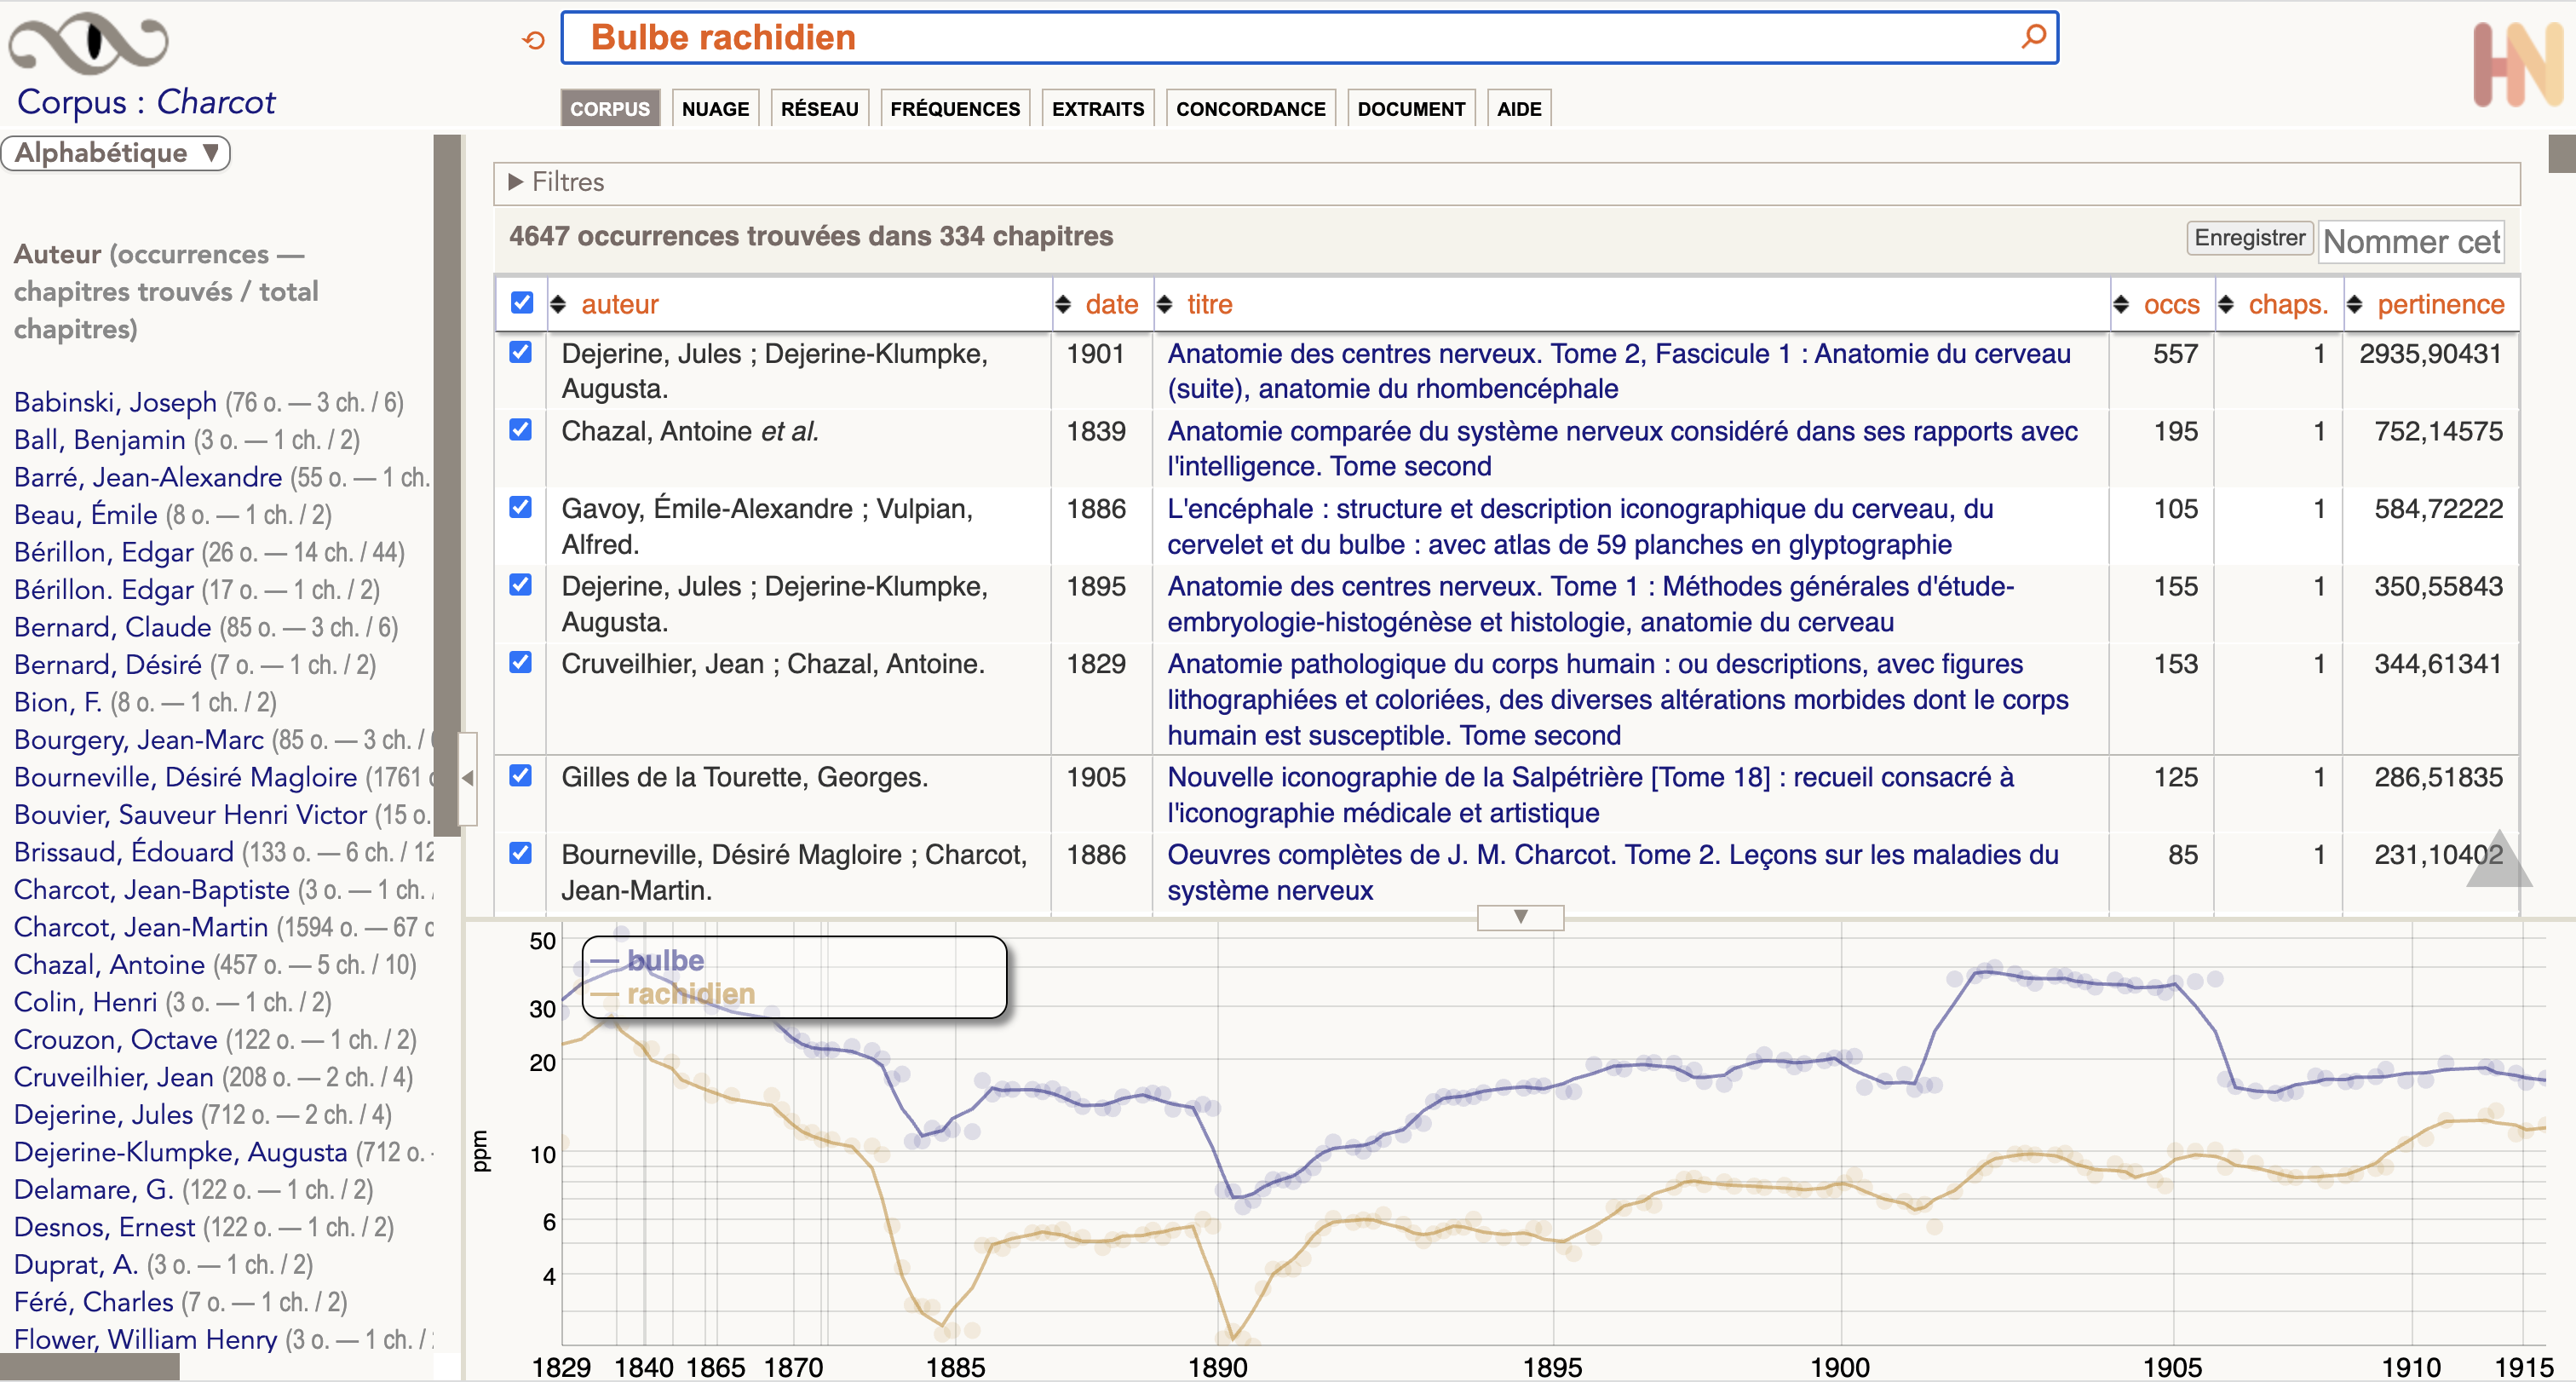
\includegraphics[width=1\textwidth]{img/bulbe_rachidien_mini.png}
    \caption{Distribution des fréquences des tokens avec la frise chronologique pour ceux constituant l'expression \og{}bulbe rachidien\fg{} (issus du corpus \og{}Charcot\fg{} et du corpus \og{}Autres\fg{}) dans le logiciel OBVIE.
    % Pour raison de visibilité, l'image originale a été agrandie, ce qui a entraîné le rapprochement des années sur l'axe de l'abscisse.
    }
    \label{fig:bulbe}
\end{figure}

Concernant l'alignement des séquences similaires aux deux corpus, \textsc{TextPair} nous a permis, par une lecture attentive, de faire des comparaisons entre les textes et de rechercher des termes au sein des passages similaires, malgré le nombre de résultats assez conséquent (\textit{cf}. la figure \ref{fig:textpair}). En raison de sa capacité de détecter les passages similaires, notamment les citations directes, les plagiats ou les réemplois, ce logiciel, ainsi qu'un autre logiciel de détection de plagiat, peuvent nous servir de \textit{baseline} pour comparer leurs résultats avec ceux proposés dans la partie \ref{methodo_stat}.

\begin{figure}[!ht]
    \centering
    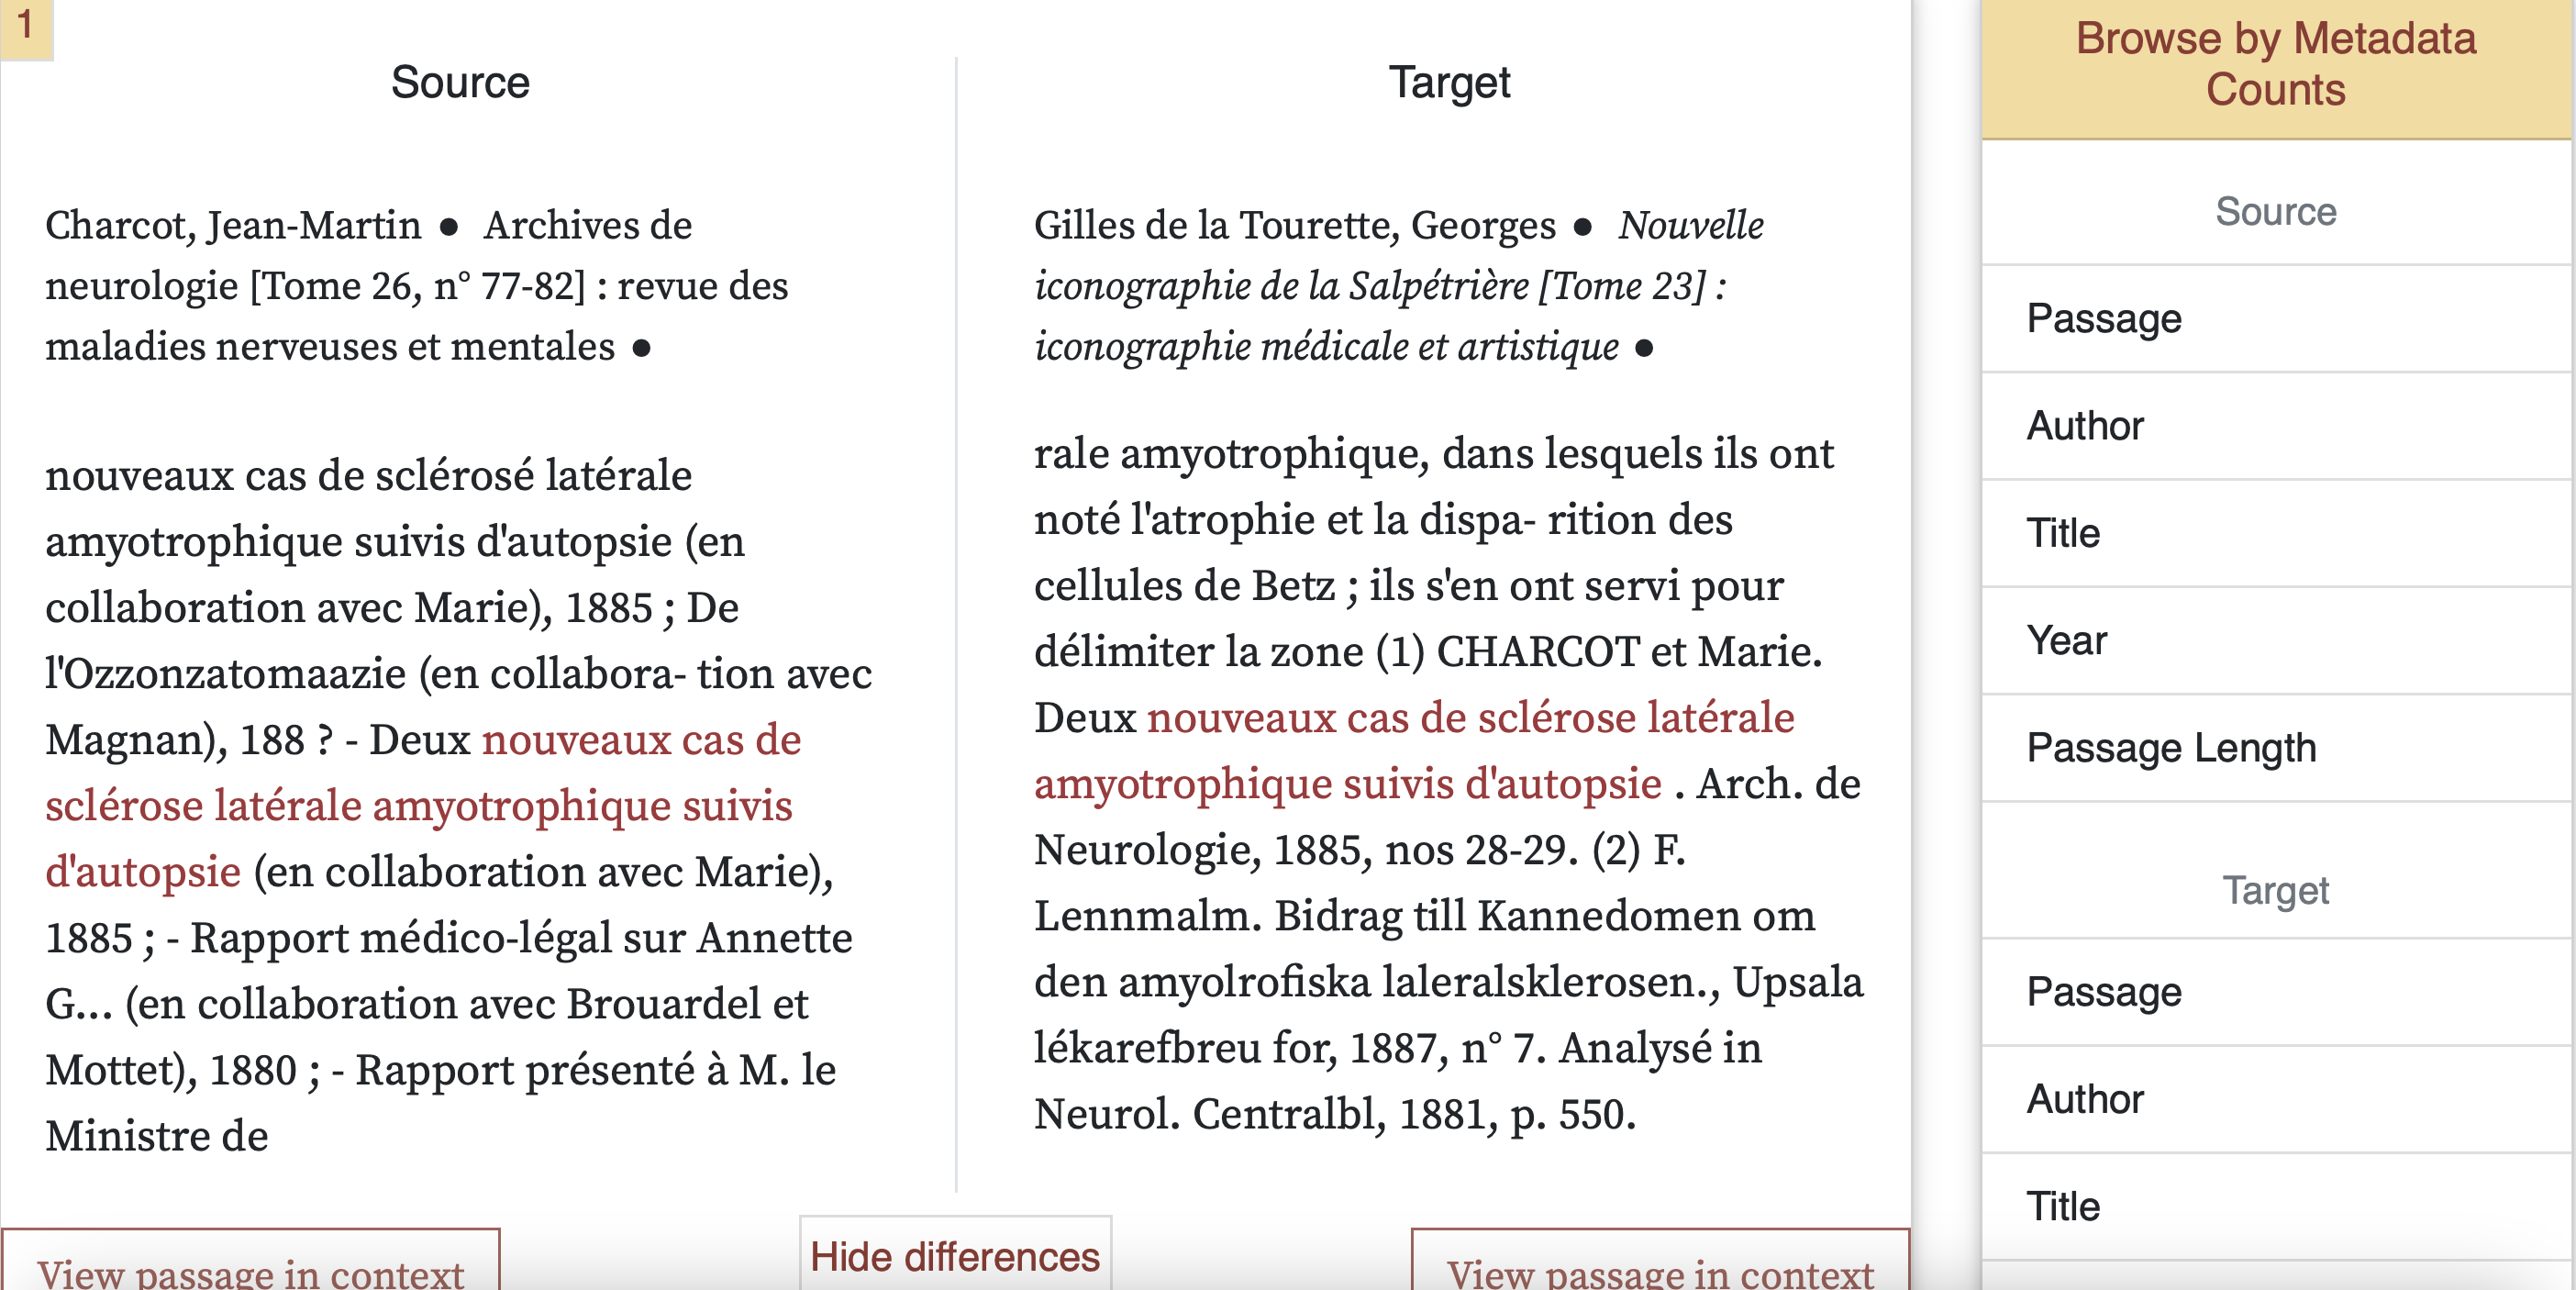
\includegraphics[width=1\textwidth]{img/textpair.png}
    \caption{Alignement et comparaison d'un texte de Charcot à celui de Georges Gilles de la Tourette (le seul résultat) en lançant la requête \textit{sclérose latérale amyotrophique}.}
    \label{fig:textpair}
\end{figure}
\section{Extraction des phrases-clés : méthodes statistiques}
\label{methodo_stat}
Afin de surmonter les limites rencontrées avec ces deux outils, nous avons proposé une nouvelle méthode pour identifier des concepts dans les deux corpus en nous basant sur le poids de leur apparition, calculé selon trois différentes mesures de pondération\footnote{Le code est disponible en ligne : \url{https://github.com/ljpetkovic/Charcot\_circulations}.} :
\begin{itemize}
\item \textsc{TF-IDF} \citep{robertson1976relevance} est une méthode qui permet d'évaluer l'importance d'un terme contenu dans un document relativement à un corpus plus large en récompensant la fréquence des termes, sans tenir compte des variations de longueur du document ;
\item \textsc{BM25} est une fonction de classement qui classe un ensemble de documents en fonction des termes de requête apparaissant dans chaque document, quelle que soit l'interrelation entre les termes de requête au sein d'un document (par exemple, leur proximité relative). Il s'agit d'une tentative d'amélioration de \textsc{TF-IDF}, notamment pour prendre en compte divers facteurs tels que la longueur du document et les problèmes engendrés par la possible saturation des termes \citep[p.~355]{robertson2009probabilistic} ;
\item \textsc{BERT} \citep{devlin2019} est un modèle pré-entraîné qui utilise l'apprentissage non-supervisé sur de grandes quantités de données textuelles pour apprendre des représentations de mots et de phrases, et comprendre le contexte et la sémantique. Il est basé sur l'architecture des \textit{transformeurs}, qui est un type de grand modèle de langue utilisé pour le \textsc{TAL}.
\end{itemize}

La liste des concepts retenus pour l'étude est composée de termes ou expressions popularisés par Charcot, comme \textit{hystérie}, \textit{sclérose latérale} etc. \citep[p.~1102]{camargo2024} \footnote{\textit{Cf.} la liste exhaustive des termes et des expressions popularisés par Charcot en annexe.}. Pour chaque entrée, nous avons pris en compte les formes du singulier et du pluriel obtenues grâce à des expressions régulières. La liste est  produite de façon supervisée et provient du croisement entre la liste des termes obtenus avec OBVIE et l'index d'une édition des \oe{}uvres complètes de \cite[pp.~493--507]{charcot1892oeuvres}, dont nous avons retiré les termes génériques (\textit{os}, \textit{cerveau}, etc.).

Comme nous pouvons l'observer sur la figure \ref{fig:bm25}, la mesure \textsc{BM25} révèle une intensification du lexique de Charcot dans le corpus \og{}Autres\fg{}. Plus précisément, tous les termes évalués sont identifiés comme plus signifiants dans le discours des \og{}Autres\fg{} que dans celui de Charcot, les scores étant plus élevés pour 14 termes (sur 14 évalués) utilisés par le réseau de Charcot. D'ailleurs, d'après le tableau \ref{tab:calculs_stat} (en annexe), c'est la seule mesure dont les valeurs témoignent clairement d'un lexique partagé entre Charcot et ses successeurs et collaborateurs, \textit{a contrario} des deux autres mesures, où le rapport en question est inversé (la grande majorité des termes étant plus pertinente dans le discours de Charcot, et son impact étant donc moins accentué). Concrètement, les termes les plus pertinents semblent être \textit{sclérose en plaque disséminées} (score 0,83), \textit{paralysie rhumatismale} (0,68), \textit{atrophie progressive} (0,53) et \textit{arthrite déformante} (0,50).

\begin{figure}[!h]
    \centering
    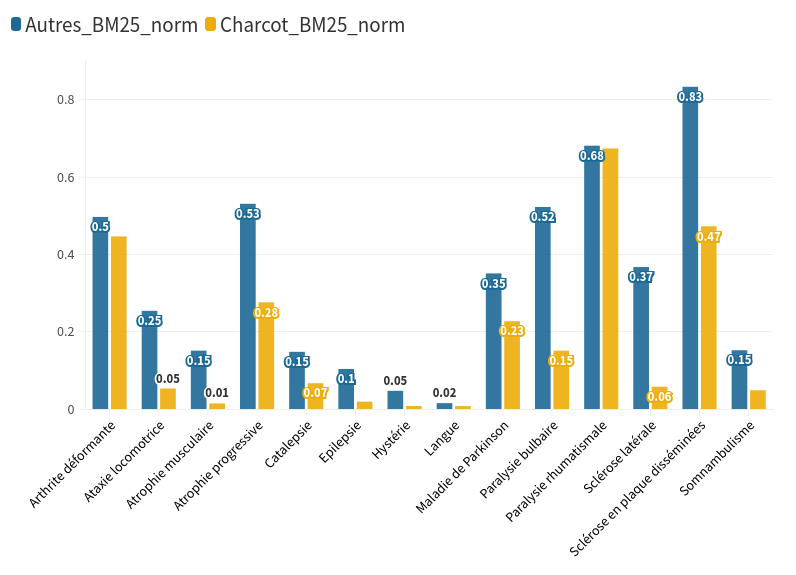
\includegraphics[width=1\textwidth]{img/Charcot_Autres_250523.png}
    \caption{Visualisation de pertinence des concepts dans les deux corpus suivant la métrique \textsc{BM25}. Les valeurs des concepts associées au corpus \og{}Autres\fg{} sont représentées en bleu, alors que celles du corpus \og{}Charcot\fg{} en jaune.}
    \label{fig:bm25}
\end{figure}

D'autre part, nous avons utilisé \textsc{BERT} pour mesurer le poids des termes dans les deux corpus. Bien que ce type de modèle ne fournisse pas directement de poids pour les mots, nous pourrions cependant en extraire des informations utiles pour estimer l'importance ou le poids des mots dans les textes. Différentes approches sont généralement utilisées pour obtenir une représentation de l'importance des mots, en exploitant les informations des plongements lexicaux et des mécanismes d'attention \citep{vaswani2023}. Pour ce travail en cours, nous avons utilisé le modèle \texttt{bert-base-multilingual-cased}. Les premiers résultats obtenus se trouvent dans le tableau \ref{tab:calculs_stat} et restent à améliorer. Cependant, nous avons observé que les termes les plus pertinents pour le discours de Charcot étaient ceux qui désignent les noms des différentes pathologies (\textit{diplopie}, \textit{myélite partielle}, \textit{état de mal épileptique}, \textit{paralysie labio-glosso-laryngée} etc.), contrairement à d'autres notions plus abstraites (\textit{vicieuses}, \textit{délire}, \textit{miracle}) qui sont prédominantes dans le corpus
\og{}Autres\fg{} (termes non renseignés dans le tableau en question). La présence de ce dernier type de notion n'est pas étonnant, étant donné que Charcot aborde la question des guérisons miraculeuses dans ses recherches\footnote{Voir notamment son \oe{}uvre \textit{La foi qui guérit} \citep{charcot1897foi}.}. 

\section{Extraction des phrases-clés : méthode à base d'apprentissage profond}
En complément de la méthode du calcul de pertinence des termes médicaux fournis de manière supervisée (partie \ref{methodo_stat}), nous exposons ici des résultats de l'approche non-supervisée pour extraire des mots/phrases-clés  pertinents à partir de nos deux corpus\footnote{\textit{Cf.} le dépôt GitHub \url{https://github.com/ljpetkovic/Charcot\_KeyBERT\_Keyphrase-Vectorizers/}.}. L'objectif de cette approche est de détecter les termes communs entre les deux corpus et de montrer la répartition des termes les plus pertinents dans le réseau de Charcot. Deux algorithmes librement disponibles sont présentés ici pour illustrer cette dernière approche : \texttt{keybert} \citep{grootendorst2023}\footnote{\url{https://maartengr.github.io/KeyBERT/}} et \texttt{keyphrase-vectorizers}\footnote{\url{https://pypi.org/project/keyphrase-vectorizers/}}.  

\subsection{Librairie \texttt{keybert}}

Cette librairie Python permet d'exploiter les plongements de mots (angl. \textit{word embeddings}) du type \textsc{BERT} pour générer des mots/phrases-clés les plus similaires à un document.
La figure \ref{fig:keybert} illustre la chaîne de traitement appliquée à nos deux corpus : 
\begin{enumerate}
\item les corpus \og Charcot \fg{} et \og Autres \fg{} sont utilisés comme les données d'entrée au format \texttt{.txt} ;
\item les documents d'entrée ont été tokenisés en phrases-clés candidates avec la fonction \texttt{CountVectorizer} ; 
\item les plongements des documents et de leurs phrases-clés candidates ont été générés par le modèle de langue \texttt{sentence-transformers} ;
\item la similarité cosinus a été calculée entre les documents d'entrée et les phrases-clés candidates, où celles avec les scores les plus élevés sont extraites.
\end{enumerate}

\begin{figure}[!h]
    \centering
    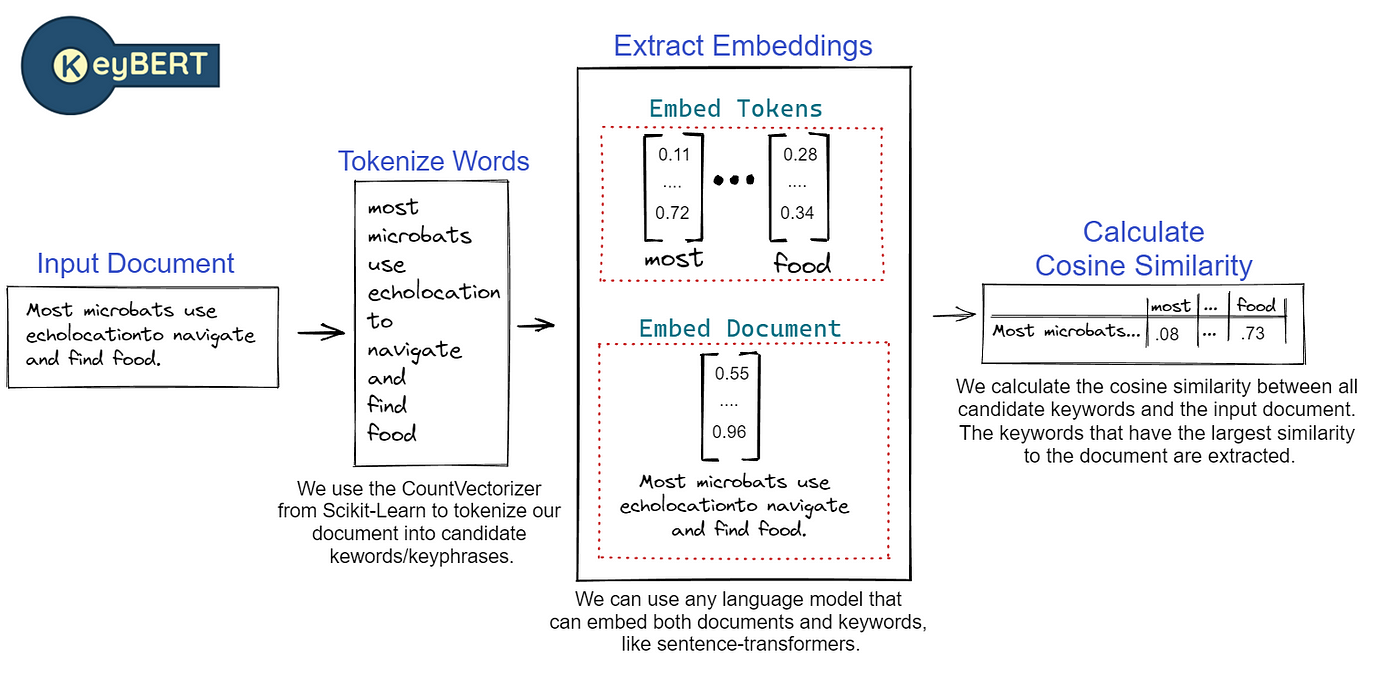
\includegraphics[width=1\textwidth]{img/keybert.png}
    \caption[Caption for LOF]{\textit{Pipeline} de la librairie \texttt{keybert}\protect\footnotemark{.}}
    \label{fig:keybert}
\end{figure}

\footnotetext{Illustration reprise de \url{https://maartengr.github.io/KeyBERT/guides/quickstart.html\#installation}.}

Une première tentative de génération des phrases-clés les plus pertinentes dans les deux corpus n'a produit que deux termes : \textsc{articulation de} [\textit{sic}] \textsc{épaule} et \textsc{paralysie faciale périphérique}. Par ailleurs, en observant les 15 phrases-clés les plus pertinentes dans le corpus \og Autres \fg{} (figure \ref{fig:keybert_autres}), nous constatons un manque de diversification des résultats et des phrases-clés qui se ressemblent (\textit{la sensibilité tactile}, \textit{sensibilité tactile au}, \textit{la sensibilité tend} etc.)\footnote{Pour assurer que les phrases-clés ne se ressemblent pas, il faut utiliser le paramètre \texttt{use\_mmr} et spécifier sa valeur entre 0 et 1.}. Un autre problème observé était la non-grammaticalité des phrases-clés extraites (\textit{sémi lunaire segment}, \textit{prière le malade} etc.), ce qui nous a incités à tester une approche plus fine, décrite dans la partie \ref{patternrank}.

\begin{figure}[!h]
    \centering
    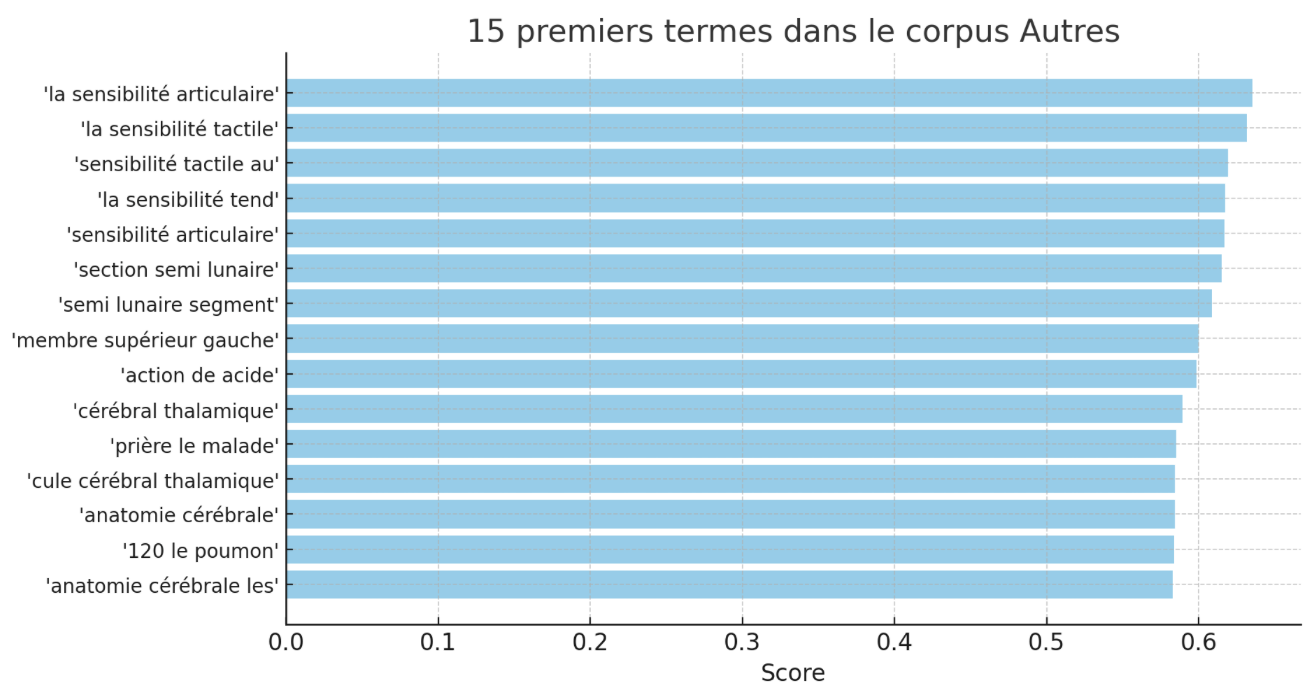
\includegraphics[width=1\textwidth]{img/keybert_autres.png}
    \caption{Répartition des 15 termes les plus pertinents dans le corpus \og{}Autres\fg{} selon \texttt{keybert}.}
    \label{fig:keybert_autres}
\end{figure}


\subsection{Approche \textit{PatternRank}}
\label{patternrank}
Cette approche exploite la librairie \texttt{keyphrase-vectorizers} qui offre la possibilité d'extraire les phrases-clés pertinentes et spécifiques à l'aide des balises de parties de discours. Cela nous a paru comme une piste intéressante, étant donné que les termes médicaux (surtout ceux plus pointus) que l'on souhaitait extraire étaient généralement des n-grammes constitués des substantifs, suivis d'un ou plusieurs adjectifs (p. ex. \textit{sclérose latérale amyotrophique}). Voici les étapes de la chaîne de traitement de l'approche \textit{PatternRank} (figure \ref{fig:patternrank}) :
\begin{enumerate}
\item les corpus \og Charcot \fg{} et \og Autres \fg{} sont utilisés comme les données d'entrée au format \texttt{.txt} ;
\item les tokens ont été extraits et étiquetés avec les balises de partie du discours et les expressions régulières \texttt{<N.*>+<ADJ.*>*} (sans utiliser le paramètre \texttt{use\_mmr}) ;
\item les tokens ont été sélectionnés selon les balises de partie de discours souhaitées et gardés comme les phrases-clés candidates ;
\item les plongements des documents et de leurs phrases-clés candidates ont été générés par le modèle de langue (en l'occurrence \texttt{flair}\footnote{\url{https://github.com/flairNLP/flair}}) ;
\item les similarités cosinus ont été calculées entre ces deux types de plongements, et les phrases-clés candidates ont été triées par ordre décroissant ;
\item les phrases-clés les plus représentatives ont été extraites.
\end{enumerate}

\begin{figure}[!h]
    \centering
    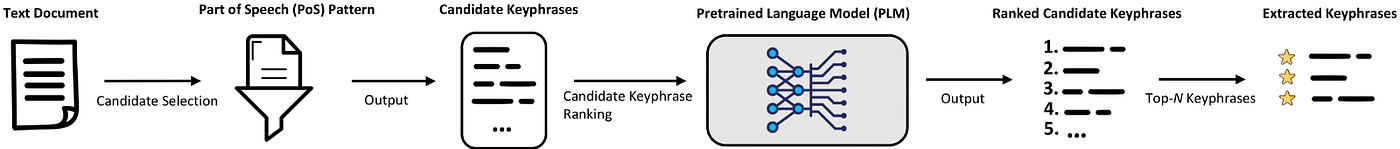
\includegraphics[width=1\textwidth]{img/patternrank_workflow.png}
    \caption{\textit{Workflow} de la méthode \textit{PatternRank} \citep[p.~2]{schopf2022}.}
    \label{fig:patternrank}
\end{figure}

La figure \ref{fig:patternrank_partage} nous informe sur les 15 termes les plus pertinents et fréquents, extraits avec la librairie \texttt{keyphrase-vectorizers}, que l'on retrouve dans les deux corpus. Malgré certains tokens tronqués, très probablement en raison d'un \textsc{OCR} imparfait (\textit{ments} $\rightarrow$ \textit{mouvements}, \textit{decins} $\rightarrow$ \textit{médecins} etc.), nous observons une diversification des résultats. Après cela, il reste la question de mieux comprendre le rôle des phrases-clés extraites dans les écrits de l'entourage de Charcot et/ou si elles sont vraiment significatives ou pas. 

\begin{figure}[!h]
    \centering
    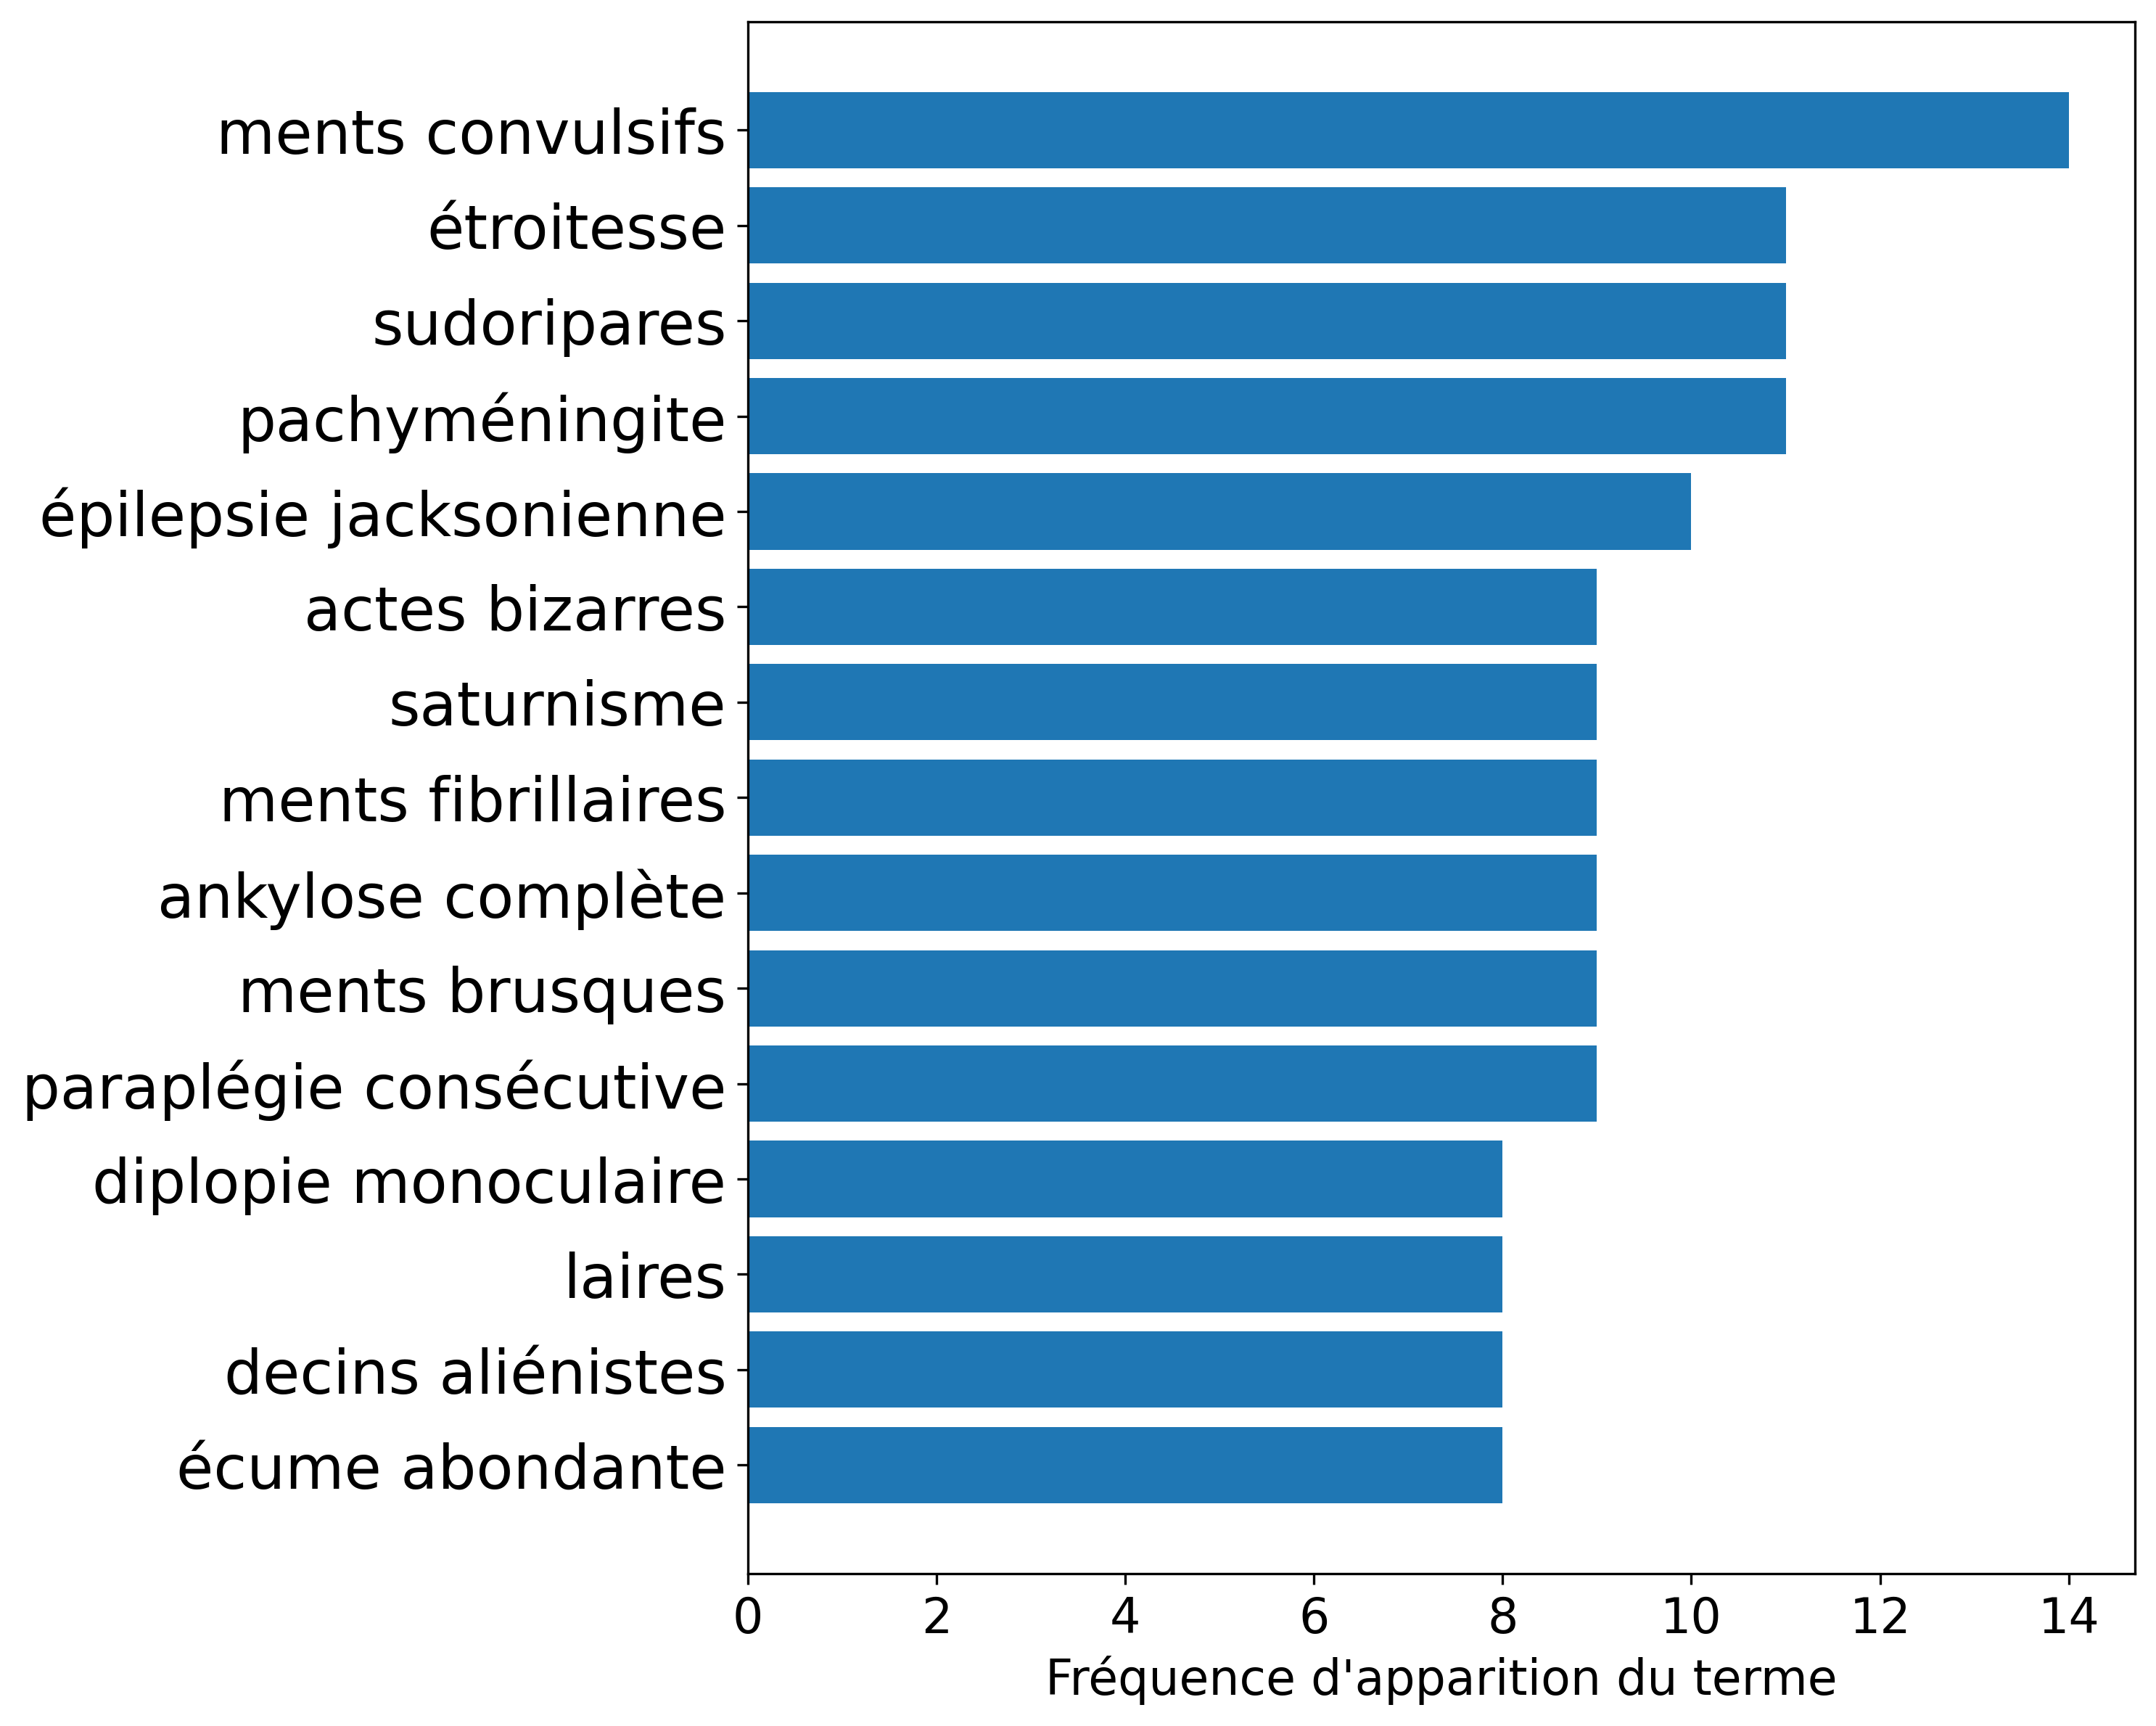
\includegraphics[width=1\textwidth]{img/termes_partages.png}
    \caption{Les 15 termes les plus fréquents partagés par les deux corpus selon \texttt{keyphrase-vectorizers}.}
    \label{fig:patternrank_partage}
\end{figure}


\chapter{Conclusion}
\chapter{Conclusion}
\minitoc
\label{conclusion}
\section{Synthèse et contributions}
%Rappel du context
Intro / Rappel Contexte

Nous avons donc pu en tirer la problématique suivante :

%Rappel des résultats

\section{Perspectives}


Discussion et perspectives


%Ne pas numéroter cette partie
\part*{Annexe}

%Rajouter la ligne "Annexes" dans le sommaire
%\addcontentsline{toc}{chapter}{Annexe}

\chapter{Annexe}



%changer le format des sections, subsections pour apparaittre sans le num de chapitre
\makeatletter
\renewcommand{\thesection}{\@arabic\c@section}
\makeatother

%recommencer la numérotation des section à "1"
\setcounter{section}{0}

%\section*{Liste des termes et expressions popularisées par Charcot}

%\addcontentsline{toc}{section}{\protect\numberline{}Liste des termes et expressions popularisées par Charcot}%
\begin{landscape}
\thispagestyle{empty}
\begin{table}[]
\centering
\begin{tabular}{|l|cccc|cccc|}
\hline
\textit{Terme} & Fréquence & \textsc{TF-IDF} & \textsc{BM25} & \textsc{BERT} & Fréquence & \textsc{TF-IDF} & \textsc{BM25} & \textsc{BERT} \\
\hline
% Data rows go here
\end{tabular}
\caption{Calcul de pertinence des concepts selon les métriques \textsc{TF-IDF}, \textsc{BM25} et \textsc{BERT} dans les corpus \og{}Charcot\fg{} et \og{}Autres\fg{}.}
\end{table}
\vfill
\raisebox{}{\makebox[\linewidth]{\thepage}}



\label{tab:calculs_stat}
\end{landscape}




\newpage

%récupérer les citation avec "/footnotemark"
\nocite{*}

%choix du style de la biblio
\addcontentsline{toc}{chapter}{References}
\bibliographystyle{apalike}
%inclusion de la biblio
\bibliography{bibliographie.bib}
%voir wiki pour plus d'information sur la syntaxe des entrées d'une bibliographie


\end{document}